%
%===================================================================================================
%
\documentclass[aspectratio=169]{beamer}
%
%===================================================================================================
%
%
%===================================================================================================
%
% Main Modular Preamble Loader
%
%===================================================================================================

%
%===================================================================================================
%
% Packages
%
%===================================================================================================

\usepackage[absolute,overlay]{textpos}

\usepackage[utf8]{inputenc}
\usepackage[T1]{fontenc}

\usepackage{amsmath}
\usepackage{amsfonts}
\usepackage{amssymb}
% the following order matter!!!
\usepackage{lmodern}
\usepackage{bm}

\usepackage{array}
\usepackage{booktabs}
\usepackage{colortbl}
\usepackage{multirow}

\usepackage{graphicx}
\usepackage{tikz}
\usepackage{pgfplots}

\usepackage{framed}
\usepackage{empheq}

\usepackage{xcolor}
\usepackage{soul}

\usepackage{hyperref}
\usepackage{pgfpages}

%\usepackage{minted}

\usepackage[most]{tcolorbox}
\tcbuselibrary{listings}

\pgfplotsset{compat=1.14}
%
%===================================================================================================
%
% TikZ Libraries
%
%===================================================================================================

\usetikzlibrary{
    arrows.meta,
    positioning,
    fit,
    calc,
    shapes.geometric,
    backgrounds,
    matrix
}

% ── Reusable TikZ styles ─────────────────────────────────────
\tikzset{
  block/.style   = {draw, rounded corners, minimum width=2.0cm,
                    minimum height=0.60cm, align=center, font=\small},
  sblock/.style  = {draw, rounded corners, minimum width=1.4cm,
                    minimum height=0.55cm, align=center, font=\small},
  token/.style   = {draw, rounded corners, minimum width=1.1cm,
                    minimum height=0.55cm, font=\small},
  arr/.style     = {->, thick, boIndigo},
  arrg/.style    = {->, gray!60, line width=0.7pt}
}

%
%===================================================================================================
%
% Custom Colors
%
%===================================================================================================

% General accents
\definecolor{accent}{RGB}{200,60,50}
\definecolor{Accent}{RGB}{240,170,0}
\definecolor{accentblue}{HTML}{457B9D}
\definecolor{accentred}{HTML}{E63946}

% Course colors
\definecolor{CourseBlue}{RGB}{47,53,163}
\definecolor{unibo}{RGB}{0,68,136}
\definecolor{uniboblue}{RGB}{0,54,132}
\definecolor{uniblue}{RGB}{0,76,147}
\definecolor{unired}{RGB}{155,0,20}
\definecolor{codebg}{RGB}{248,248,248}
\definecolor{lightblue}{RGB}{220,235,250}

% Code colors
\definecolor{codebg}{rgb}{0.97,0.97,0.97}
\definecolor{codeborder}{rgb}{0.8,0.8,0.8}

% Neural-network / layer colors
\definecolor{w1col}{RGB}{255,180,0}
\definecolor{w2col}{RGB}{180,90,30}
\definecolor{b1col}{RGB}{0,255,0}
\definecolor{layer1violet}{HTML}{800080}
\definecolor{layer2red}{HTML}{FF0000}
\definecolor{updategreen}{HTML}{228B22}

% Financial colors
\definecolor{finblue}{RGB}{0,51,102}
\definecolor{fingray}{RGB}{100,100,100}
\definecolor{fingreen}{RGB}{0,100,0}
\definecolor{finred}{RGB}{178,34,34}

% Semantic colors
\definecolor{darkgreen}{RGB}{0,120,60}
\definecolor{DeepRed}{RGB}{180,45,45}
\definecolor{Forest}{RGB}{34,120,70}

% Light background colors
\definecolor{lightblue}{RGB}{210,230,250}
\definecolor{lightgreen}{RGB}{210,245,210}
\definecolor{lightorange}{RGB}{255,235,205}
\definecolor{lightred}{RGB}{255,220,220}
\definecolor{lightyellow}{RGB}{255,255,210}

% Soft background colors
\definecolor{SoftBlue}{RGB}{225,235,255}
\definecolor{SoftGray}{RGB}{245,245,245}
\definecolor{SoftGreen}{RGB}{228,243,232}
\definecolor{SoftOrange}{RGB}{255,244,224}

% Modern palette
\definecolor{navy}{RGB}{15,27,61}
\definecolor{deepblue}{RGB}{22,38,83}
\definecolor{midblue}{RGB}{30,58,110}
\definecolor{teal}{RGB}{13,148,136}
\definecolor{lightgray}{RGB}{148,163,184}
\definecolor{ice}{RGB}{202,220,252}
\definecolor{gold}{RGB}{245,158,11}
\definecolor{coral}{RGB}{249,115,22}
\definecolor{darktext}{RGB}{30,41,59}
\definecolor{offwhite}{RGB}{240,244,250}
\definecolor{boIndigo}{RGB}{55,0,153}

\definecolor{NavyBlue}{RGB}{20,40,100}
\definecolor{SteelBlue}{RGB}{70,130,180}
\definecolor{LightGray}{RGB}{245,245,250}
\definecolor{AccentGold}{RGB}{210,160,30}

\definecolor{futC} {gray}{0.60}
\definecolor{actC} {RGB}{15, 82, 186}
\definecolor{doneC}{RGB}{25, 25,  25}

\definecolor{GateOrange}{RGB}{230,120,0}
\definecolor{GatePurple}{RGB}{110,0,150}
\definecolor{CellGold}{RGB}{160,120,0}

% Alias
\colorlet{bolight}{boIndigo!10}
\colorlet{bodark}{boIndigo!85!black}
\colorlet{actFill}{actC!10}   % light-blue cell background when active


%
%===================================================================================================
%
% Beamer Theme and Style
%
%===================================================================================================

\usetheme{Madrid}
\usecolortheme{default}

%
%===================================================================================================
%
% Beamer Color Customization
%
%===================================================================================================

\setbeamercolor{title}{fg=white,bg=CourseBlue}
\setbeamercolor{frametitle}{fg=white,bg=CourseBlue}
\setbeamercolor{structure}{fg=CourseBlue}

\setbeamercolor{block title}{fg=white,bg=CourseBlue}
\setbeamercolor{block body}{fg=black,bg=SoftGray}

\setbeamercolor{item projected}{fg=white,bg=CourseBlue}

\setbeamercolor{section in head/foot}{fg=white,bg=CourseBlue}
\setbeamercolor{subsection in head/foot}{fg=white,bg=CourseBlue!80!black}
\setbeamercolor{author in head/foot}{fg=white,bg=CourseBlue!90!black}
\setbeamercolor{title in head/foot}{fg=white,bg=CourseBlue!70!black}
\setbeamercolor{date in head/foot}{fg=white,bg=CourseBlue!90!black}

%
%===================================================================================================
%
% Navigation Symbols and Itemize Style
%
%===================================================================================================

\setbeamertemplate{navigation symbols}{}

\setbeamertemplate{itemize item}{\color{CourseBlue}$\blacktriangleright$}
\setbeamertemplate{itemize subitem}{\color{CourseBlue}$\bullet$}
%
%===================================================================================================
%
% Mathematical Macros
%
%===================================================================================================

\newcommand{\vect}[1]{\bm{#1}}
\newcommand{\R}{\mathbb{R}}

\newcommand{\bx}{\bm{x}}
\newcommand{\bh}{\bm{h}}
\newcommand{\bw}{\bm{w}}
\newcommand{\bW}{\bm{W}}
\newcommand{\bb}{\bm{b}}
\newcommand{\diag}{\operatorname{diag}}

\newcommand{\vw}{\mathbf{w}}
\newcommand{\vwt}{\tilde{\mathbf{w}}}
%
%===================================================================================================
%
% Text and Highlighting Macros
%
%===================================================================================================

\newcommand{\soft}[1]{\textcolor{CourseBlue}{\textbf{#1}}}

\newcommand{\highlight}[1]{%
    \colorbox{yellow!25}{$\displaystyle #1$}
}

%
%===================================================================================================
%
% Beamer-Compatible Highlight Fix for the soul Package
%
%===================================================================================================

\makeatletter
\let\HL\hl
\renewcommand\hl{%
  \let\set@color\beamerorig@set@color
  \let\reset@color\beamerorig@reset@color
  \HL}
\makeatother

%
%===================================================================================================
%
% Custom Intuition Box
%
%===================================================================================================

\newcommand{\intuition}[1]{%
  \vspace{4pt}
  \begin{tikzpicture}
    \node[
        fill=offwhite,
        rounded corners=4pt,
        inner sep=6pt,
        text width=0.92\textwidth
    ] {%
      \textcolor{teal}{\textbf{Intuition:}} 
      \textcolor{darktext}{\small #1}
    };
  \end{tikzpicture}
}


\newcommand{\dmodel}{d_{\mathrm{model}}}
\newcommand{\dff}{d_{\mathrm{ff}}}
\newcommand{\dk}{d_k}
\newcommand{\dv}{d_v}

% ─────────────────────────────────────────────────────────────────────
%  \drawcell{cx}{cy}{border-color}{fill-color}
%  Draws the RNN cell rectangle + 3 neuron circles at (cx, cy).
% ─────────────────────────────────────────────────────────────────────
\newcommand{\drawcell}[4]{%
  \fill[#4, rounded corners=3pt]
    ({#1-0.68},{#2-1.10}) rectangle ({#1+0.68},{#2+1.10});
  \draw[color=#3, line width=1.5pt, rounded corners=3pt]
    ({#1-0.68},{#2-1.10}) rectangle ({#1+0.68},{#2+1.10});
  \draw[color=#3, line width=0.9pt] (#1,{#2+0.55}) circle(0.21);
  \draw[color=#3, line width=0.9pt] (#1, #2)        circle(0.21);
  \draw[color=#3, line width=0.9pt] (#1,{#2-0.55}) circle(0.21);
}
% Bold vectors shortcut (match existing notation)
\newcommand{\vct}[1]{\bm{#1}}

%
%===================================================================================================
%
\title{Chapter 4 -- The Attention Mechanism and the Transformer Architecture}
\subtitle{Advanced Machine Learning for Finance}
\author{Giovanni Della Lunga}
\institute{University of Bologna}
\date{April-May 2026}
%
%===================================================================================================
%
\AtBeginSection[]{
\begin{frame}
\vfill
\centering
\begin{beamercolorbox}[sep=10pt,center,shadow=true,rounded=true]{title}
\usebeamerfont{title}\insertsectionhead\par
\end{beamercolorbox}
\vfill
\end{frame}
}
%
%===================================================================================================
%
\begin{document}
%
%===================================================================================================
%
\begin{frame}
    \titlepage
\end{frame}
%__________________________________________________________________________
%
\section{Introduction}
%__________________________________________________________________________
%
\begin{frame}{Where We Are}
  \textbf{Lesson 1 – Classical NLP}\\[0.2em]
  Bag-of-words, TF-IDF, cosine similarity: sparse, high-dimensional, no word-order,
  no semantics beyond co-occurrence counts.

  \vspace{0.6em}
  \textbf{Lesson 2 – Neural Networks, Embeddings, and Tokenization}\\[0.2em]
  Perceptron $\to$ gradient learning $\to$ Word2Vec\,/\,GloVe: dense, distributed,
  encode semantic similarity, but \emph{static} – one vector per word regardless of
  context.\\
  BPE and sub-word tokenization: how raw text becomes token IDs.

  \vspace{0.6em}
  \begin{alertblock}{Today's question}
    How do we move from a single fixed vector per word to representations that capture
    meaning in context, and what is the architecture that makes this possible at scale?
  \end{alertblock}
\end{frame}
%
%..................................................................
%
\begin{frame}{Lesson 3 – Outline}
  \begin{columns}[t]
    \begin{column}{0.48\textwidth}
      \textbf{Part I – The Problem}
      \begin{itemize}
        \item From static to contextual embeddings
        \item The polysemy problem in finance
        \item Early attempts: RNNs and LSTMs
      \end{itemize}
      \vspace{0.5em}
      \textbf{Part II – The Attention Mechanism}
      \begin{itemize}
        \item Intuition: attention as soft lookup
        \item Similarity scores and scaled dot-product attention
        \item A step-by-step walkthrough
        \item Why scale by $\sqrt{d_k}$?
        \item Self-attention and why it works
      \end{itemize}
    \end{column}
    \begin{column}{0.48\textwidth}
      \textbf{Part II (cont.)}
      \begin{itemize}
        \item Multi-head attention
        \item Attention: interpretation and caution
      \end{itemize}
      \vspace{0.5em}
      \textbf{Part III – Positional Encoding}
      \begin{itemize}
        \item Why do we need positional information?
        \item Sinusoidal positional encoding
      \end{itemize}
      \vspace{0.5em}
      \textbf{Part IV – The Transformer}
      \begin{itemize}
        \item Full architecture overview
        \item Residual connections \& layer norm
        \item Feed-forward sub-layer
        \item Masked attention \& the decoder
      \end{itemize}
    \end{column}
  \end{columns}
\end{frame}
%__________________________________________________________________________
%
\section{From Static to Contextual Embeddings}
%__________________________________________________________________________
%
\begin{frame}{The Polysemy Problem}
  \begin{exampleblock}{Example}
    \begin{itemize}
      \item ``The bank raised interest rates.''
      \item ``We walked along the river bank.''
    \end{itemize}
  \end{exampleblock}

  Word2Vec assigns one vector to ``bank''. It conflates all senses into a single point
  in semantic space.

  \vspace{0.5em}
  \textbf{What we need:} a representation that depends on the surrounding words – a
  function
  \[
    f(\text{word},\,\text{context}),\quad\text{not just }f(\text{word}).
  \]

  \begin{block}{Financial relevance}
    ``spread'', ``yield'', ``default'', ``call'', ``exposure'' – domain-specific
    polysemy is pervasive in finance.  A model that cannot disambiguate these in context
    is fundamentally limited for financial NLP.
  \end{block}
\end{frame}
%
%..................................................................
%
\begin{frame}{Early Attempts: RNNs and LSTMs}
  Recurrent Neural Networks process tokens sequentially, passing a hidden state forward:
  \[
    h_t = \sigma\!\bigl(W_h h_{t-1} + W_x x_t + b\bigr).
  \]
  Each $h_t$ is contextual: it depends on the words seen so far.

  \vspace{0.4em}
  Long Short-Term Memory (LSTM) adds gating mechanisms to control information flow and
  alleviate vanishing gradients.

  \vspace{0.4em}
  \begin{alertblock}{Key limitations}
    \begin{itemize}
      \item Sequential processing: cannot parallelise across positions – training is
            slow.
      \item Long-range dependencies: despite gates, information from distant positions
            degrades.
    \end{itemize}
  \end{alertblock}
  These limitations motivated the search for a fundamentally different architecture.
\end{frame}
%
%..................................................................
%
\begin{frame}{Contextual Embeddings: The Core Idea}
  \begin{columns}[c]
    \begin{column}{0.42\textwidth}
      \vspace{-.75cm}
      \begin{block}{Word2Vec}
        \centering\vspace{0.3em}
        ``bank'' $\mapsto$ $e_{\text{bank}}$\\[0.5em]
        {\small same vector always}\vspace{0.3em}
      \end{block}
    \end{column}
    \begin{column}{0.52\textwidth}
      \begin{block}{Contextual Model}
        \centering\vspace{0.3em}
        ``The bank raised rates'' $\;\to\;$ $h^{(1)}_{\text{bank}}$\\[0.3em]
        ``Along the river bank'' $\;\to\;$ $h^{(2)}_{\text{bank}}$\\[0.5em]
        {\small different vectors}\vspace{0.3em}
      \end{block}
    \end{column}
  \end{columns}

  \vspace{1em}
  A contextual embedding model produces a \textbf{different vector} for each occurrence
  of a word, conditioned on its full sentential context.

  \vspace{0.5em}
  The Transformer architecture achieves this via \textbf{attention}, without any
  sequential recurrence.
\end{frame}
%__________________________________________________________________________
%
\section{The Attention Mechanism}
%__________________________________________________________________________
%
\begin{frame}{Attention: The Basic Problem}
  Before introducing new terminology, start from the practical question:

  \vspace{0.4em}
  \begin{center}
    \itshape For each word, which other words should influence its meaning?
  \end{center}
  \vspace{0.4em}

  In the sentence ``The Fed raised rates'', the vector for \textit{rates} should be
  influenced strongly by \textit{Fed} and \textit{raised}, and only weakly by \textit{The}.

  \vspace{0.3em}
  \begin{center}
  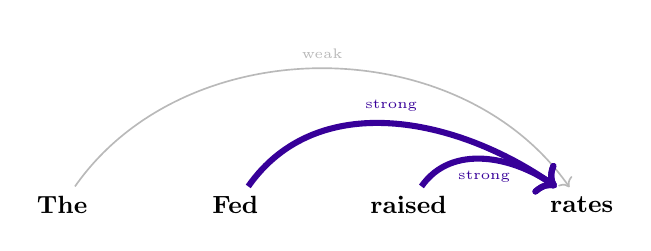
\begin{tikzpicture}
    \node (The)    at (0,0)   {\small\textbf{The}};
    \node (Fed)    at (2.2,0) {\small\textbf{Fed}};
    \node (raised) at (4.4,0) {\small\textbf{raised}};
    \node (rates)  at (6.6,0) {\small\textbf{rates}};

    \draw[->, gray!55, line width=0.6pt]
      (The) to[out=55,in=125] node[above,font=\tiny]{weak}   (rates);
    \draw[->, boIndigo, line width=2.2pt]
      (Fed) to[out=55,in=145] node[above,font=\tiny]{strong} (rates);
    \draw[->, boIndigo, line width=2.2pt]
      (raised) to[out=55,in=145] node[below,font=\tiny]{strong} (rates);
  \end{tikzpicture}
  \end{center}

  \vspace{0.2em}
  Attention is the mechanism that \textbf{learns} these strengths automatically and uses
  them to build a new, context-dependent vector for each token.
\end{frame}
%
%..................................................................
%
\begin{frame}{Attention as Soft Selection}
  A simple way to think about attention is \textbf{soft selection}:
  \begin{enumerate}
    \item Pick the token we want to update, for example \textit{rates}.
    \item Compare it with every token in the sentence.
    \item Give each comparison a numerical score.
    \item Convert the scores into weights that sum to one.
    \item Build the new vector as a weighted mixture of information.
  \end{enumerate}

  \vspace{0.3em}
  \begin{center}
  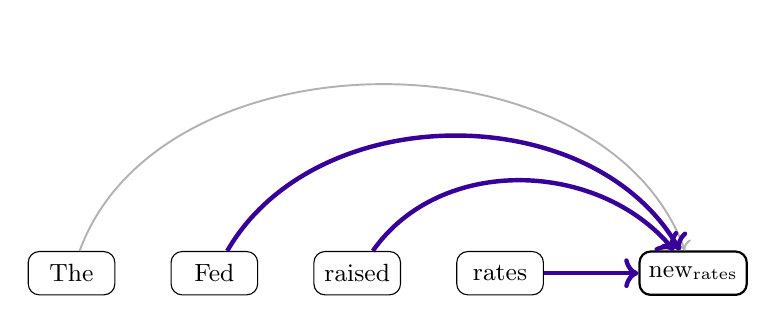
\begin{tikzpicture}[token]
    \node[token] (T) {The};
    \node[token, right=0.7cm of T] (F) {Fed};
    \node[token, right=0.7cm of F] (R) {raised};
    \node[token, right=0.7cm of R] (r) {rates};
    \node[token, right=1.2cm of r, draw, thick] (nr) {new$_{\text{rates}}$};

    \draw[arrg] (T) to[out=70,in=110] (nr);
    \draw[arr, line width=1.6pt] (F) to[out=60,in=120] (nr);
    \draw[arr, line width=1.6pt] (R) to[out=55,in=130] (nr);
    \draw[arr, line width=1.6pt] (r) -- (nr);
  \end{tikzpicture}
  \end{center}

  The arrows will become numerical weights.
\end{frame}
%
%..................................................................
%
\begin{frame}{A First Attempt: Similarity-Based Mixing}
  Simplest idea: use the dot product between embedding vectors as a measure of how
  much two tokens are related.  Tokens whose embeddings are similar (high dot product)
  should exchange more information; dissimilar tokens should exchange less.

  For each token $i$, compute a new representation $z_i$ as a weighted average of all
  input embeddings:
  \[
    z_i = \sum_{j=1}^{n}\alpha_{ij}\,x_j, \qquad
    \alpha_{ij} = \frac{\exp\!\bigl(x_i^\top x_j\bigr)}
                       {\displaystyle\sum_{j'}\exp\!\bigl(x_i^\top x_{j'}\bigr)}.
  \]

  \begin{block}{What is happening here?}
    \begin{itemize}
      \item $x_i^\top x_j$ measures the similarity between tokens $i$ and $j$ in the
            embedding space.
      \item The softmax converts raw similarities into weights that sum to~1.
      \item The output $z_i$ is a blend of all input embeddings, with more weight on
            the most similar ones.
    \end{itemize}
  \end{block}
\end{frame}
%
%..................................................................
%
\begin{frame}{Concrete Example: Raw Similarity Attention}
  \begin{columns}[t]
    \begin{column}{0.52\textwidth}
      Consider: ``The Fed raised rates''. Compute the dot product of each token's
      embedding with every other.

      \vspace{0.5em}
      \begin{center}
      {\small
      \begin{tabular}{lrrrr}
        \toprule
               & The  & Fed  & raised & rates \\
        \midrule
        The    & 3.0  & 0.1  & 0.0    & 0.3   \\
        Fed    & 0.1  & 3.2  & 1.8    & 2.1   \\
        raised & 0.0  & 1.8  & 3.5    & 2.7   \\
        rates  & 0.3  & 2.1  & 2.7    & 3.4   \\
        \bottomrule
      \end{tabular}}
      \end{center}
      {\small Raw dot-product scores $s_{ij} = x_i^\top x_j$.}
    \end{column}
    \begin{column}{0.44\textwidth}
      \begin{itemize}
        \item Diagonal is large: every word is most similar to itself.
        \item ``rates'' and ``raised'': score 2.7 – semantically related words have
              higher similarity.
        \item ``The'' and ``rates'': score 0.3 – function words are distant from
              content words.
      \end{itemize}
      \vspace{0.4em}
      After softmax, the new embedding of ``rates'' would be a blend dominated by
      itself and ``raised'' – already a rough contextualisation.
    \end{column}
  \end{columns}
\end{frame}
%
%..................................................................
%
\begin{frame}{Introducing the Query, Key, Value Representation}
\small
  Consider one token, \textit{rates}.  It gets a query vector $q_{\text{rates}}$;
  every token gets a key vector $k_j$.  The raw relevance score is a scalar product:
  \[
    s_{\text{rates},j} = q_{\text{rates}}^\top k_j.
  \]
  The new vector is then a weighted sum of value vectors:
  \[
    z_{\text{rates}} = \sum_j \alpha_{\text{rates},j}\,v_j.
  \]
  The words \emph{query}, \emph{key}, and \emph{value} are just names for three roles
  in the soft lookup.

  \begin{columns}[t]
    \begin{column}{0.30\textwidth}
      \begin{block}{Query}
        What the current token is looking for.\\[0.3em]
        For ``rates'': what context helps explain me?
      \end{block}
    \end{column}
    \begin{column}{0.30\textwidth}
      \begin{block}{Key}
        What each token advertises about itself.\\[0.3em]
        ``Fed'' advertises central-bank information.
      \end{block}
    \end{column}
    \begin{column}{0.30\textwidth}
      \begin{block}{Value}
        The information that will be passed on if that token is relevant.\\[0.3em]
        The content contributed by ``Fed''.
      \end{block}
    \end{column}
  \end{columns}
\end{frame}
%
%..................................................................
%
\begin{frame}{Query, Key, Value: A Quick Resume}
  \begin{center}

\includegraphics[scale=.4]{../05-pictures/chapter-04_pic_0.png} 
  \end{center}
ter\end{frame}
%
%..................................................................
%
\begin{frame}{Why Raw Similarity Is Not Enough}
  The simple dot-product approach works as a first approximation, but it has three
  fundamental limitations.

  \vspace{0.4em}
  \begin{alertblock}{Limitation 1: The same vector plays two roles}
    The embedding $x_i$ must simultaneously serve as:
    \begin{itemize}
      \item the \emph{address}: what to match on – ``am I relevant to you?''
      \item the \emph{content}: what to transmit – ``here is my information''
    \end{itemize}
    But these are different functions.  A word might be highly relevant to another
    without being semantically similar to it.
  \end{alertblock}

  \vspace{0.4em}
  \begin{alertblock}{Limitation 2: Similarity is symmetric}
    $x_i^\top x_j = x_j^\top x_i$, but relevance is often asymmetric:
    ``rates'' should attend strongly to ``raised'' to understand what happened, but
    ``raised'' may need ``Fed'' more than ``rates''.
  \end{alertblock}
\end{frame}
%
%..................................................................
%
\begin{frame}{Why Raw Similarity Is Not Enough}
  \begin{alertblock}{Limitation 3: No learning}
    Raw dot products use the embedding space as-is.  The model cannot learn
    task-specific notions of relevance – what matters for sentiment analysis is
    different from what matters for named entity recognition.
  \end{alertblock}
\end{frame}
%
%..................................................................
%
\begin{frame}{The Solution: Three Separate Learned Projections}
  The fix is elegant: instead of comparing raw embeddings, project each embedding into
  three separate spaces using learned weight matrices:
  \[
    q_i = W^Q x_i, \qquad k_i = W^K x_i, \qquad v_i = W^V x_i.
  \]

  \begin{block}{Each projection has a distinct role}
    \begin{itemize}
      \item $Q$: what this position should look for;
      \item $K$: how this position should be matched by other tokens;
      \item $V$: what information this position contributes to the output.
    \end{itemize}
  \end{block}

  The key point is that the model learns the comparison space and the content space
  \textbf{separately}.
\end{frame}
%
%..................................................................
%
\begin{frame}{The Solution: Three Separate Learned Projections}
  What changed compared to the simple version?

  \vspace{0.5em}
  \begin{columns}[t]
    \begin{column}{0.44\textwidth}
      \begin{block}{Before}
        \centering\vspace{0.3em}
        $s_{ij} = x_i^\top x_j$\\[0.4em]
        {\small Same vector, dual role, symmetric, fixed.}
        \vspace{0.3em}
      \end{block}
    \end{column}
    \begin{column}{0.44\textwidth}
      \begin{block}{Now}
        \centering\vspace{0.3em}
        $s_{ij} = q_i^\top k_j$\\[0.4em]
        {\small Different projections, asymmetric, learnable.}
        \vspace{0.3em}
      \end{block}
    \end{column}
  \end{columns}

  \vspace{0.8em}
  And the content transmitted is $v_j$, not $x_j$ – relevance is decoupled from
  content.
\end{frame}
%
%..................................................................
%
\begin{frame}{Scaled Dot-Product Attention}
  Given matrices $Q, K, V \in \mathbb{R}^{n \times d_k}$:
  \[
    \mathrm{Attention}(Q,K,V)
    = \mathrm{softmax}\!\left(\frac{QK^\top}{\sqrt{d_k}}\right)V.
  \]

      \textbf{Step by step:}
      \begin{enumerate}
        \item Compute all pairwise scalar products:
              $S = QK^\top$, with $S_{ij} = q_i^\top k_j$.
        \item Scale by $\sqrt{d_k}$ to prevent softmax saturation.
        \item Apply softmax row-wise $\to$ attention weights $\alpha_{ij}$.
        \item Output $=$ weighted sum of value vectors.
      \end{enumerate}
  \end{frame}
%
%..................................................................
%
\begin{frame}{From Hard Lookup to Soft Lookup}
\small
  Now that the full formulation has been introduced, we can reinterpret attention as a
  learnable version of lookup.
  \vspace{-.5cm}
  \begin{columns}[t]
    \begin{column}{0.44\textwidth}
      \begin{block}{Hard lookup: classical dictionary}
        \begin{itemize}
          \item A query matches exactly one key.
          \item It returns one associated value.
          \item The choice is discrete: the rule is fixed by exact matching.
        \end{itemize}
      \end{block}
    \end{column}
    \begin{column}{0.50\textwidth}
      \begin{block}{Soft lookup: attention}
        \begin{itemize}
          \item A token can match all other tokens to varying degrees.
          \item It returns a weighted average of their value vectors.
          \item The matching rule is learned through $W^Q$, $W^K$, and $W^V$.
        \end{itemize}
      \end{block}
    \end{column}
  \end{columns}

  \begin{block}{Why this is learnable}
    The scalar products $q_i^\top k_j$ produce the scores, but the vectors $q_i$,
    $k_j$, and $v_j$ are themselves produced by learned matrices.  During training,
    gradient descent adjusts these matrices so that the model learns what to compare
    and what information to pass on.
  \end{block}
\end{frame}
%
%..................................................................
%
\begin{frame}{Walkthrough: Setting Up the Problem}
\small
  Let us trace the attention computation on a short sentence:
  \begin{center}
    \textit{``The Fed raised rates''}
  \end{center}
  After tokenization and embedding, we have four input vectors
  $x_1, \ldots, x_4 \in \mathbb{R}^d$.

  For this walkthrough, suppose $d = d_k = 4$ (toy dimensions).

  \vspace{0.5em}
  \textbf{Step 0:} Move from the plain-language roles to their vector form.  For every
  token, the model creates three learned views:
  \[
    Q = XW^Q, \quad K = XW^K, \quad V = XW^V.
  \]
  \begin{itemize}
    \item Each row of $Q$ is the \emph{query} for that token: ``what am I looking for?''
    \item Each row of $K$ is the \emph{key}: ``what do I have that may match?''
    \item Each row of $V$ is the \emph{value}: ``what information will I pass on if
          selected?''
  \end{itemize}
\end{frame}
%
%..................................................................
%
\begin{frame}{Walkthrough: Computing Attention Scores}
  \textbf{Step 1:} Compute all pairwise scores $S = QK^\top$:
  \[
    S = QK^\top =
    \begin{pmatrix}
      q_1^\top k_1 & q_1^\top k_2 & q_1^\top k_3 & q_1^\top k_4 \\
      q_2^\top k_1 & q_2^\top k_2 & q_2^\top k_3 & q_2^\top k_4 \\
      q_3^\top k_1 & q_3^\top k_2 & q_3^\top k_3 & q_3^\top k_4 \\
      q_4^\top k_1 & q_4^\top k_2 & q_4^\top k_3 & q_4^\top k_4
    \end{pmatrix}.
  \]

  \begin{columns}[t]
    \begin{column}{0.52\textwidth}
      \begin{center}
      {\small
      \begin{tabular}{lrrrr}
        \toprule
               & The  & Fed  & raised & rates \\
        \midrule
        The    & 2.1  & 0.5  & 0.3    & 0.1   \\
        Fed    & 0.4  & 1.8  & 1.2    & 1.5   \\
        raised & 0.2  & 1.0  & 2.0    & 1.6   \\
        rates  & 0.1  & 1.4  & 1.5    & 2.2   \\
        \bottomrule
      \end{tabular}}
      \end{center}
    \end{column}
    \begin{column}{0.44\textwidth}
      \begin{itemize}
        \item Entry $(i,j)$: how much does token $i$'s query match token $j$'s key.
        \item Example: ``rates'' attends strongly to ``Fed'' (1.4) and ``raised''
              (1.5) – financially meaningful.
      \end{itemize}
    \end{column}
  \end{columns}
\end{frame}
%
%..................................................................
%
\begin{frame}{Walkthrough: Scaling and Softmax}
  \textbf{Step 2:} Divide by $\sqrt{d_k}$ (here $\sqrt{4}=2$):
  \[
    S' = \frac{S}{\sqrt{d_k}}
  \]
  For example, row ``rates'': $(0.05,\;0.70,\;0.75,\;1.10)$.

  \vspace{0.5em}
  \textbf{Step 3:} Apply softmax row-wise to get attention weights $\alpha$:
  \[
    \alpha_{ij} =
    \frac{\exp(S'_{ij})}{\displaystyle\sum_{j'}\exp(S'_{ij'})}.
  \]
  For the row corresponding to ``rates'':
  \[
    \alpha_{\text{rates}} = (0.13,\;0.25,\;0.26,\;0.36).
  \]
\end{frame}
%
%..................................................................
%
\begin{frame}{Walkthrough: Computing the Output}
  \textbf{Step 4:} The output for each token is the weighted sum of value vectors:
  \[
    z_i = \sum_{j=1}^{n} \alpha_{ij}\,v_j.
  \]

  \begin{center}
  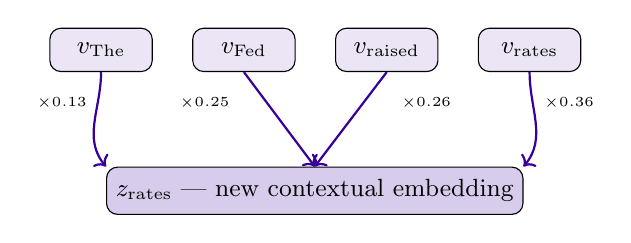
\begin{tikzpicture}[
    vbox/.style={draw, fill=bolight, rounded corners,
                 minimum width=1.3cm, minimum height=0.55cm, font=\small},
    node distance=0.8cm
  ]
    \node[vbox] (vT) {$v_{\text{The}}$};
    \node[vbox, right=0.5cm of vT] (vF) {$v_{\text{Fed}}$};
    \node[vbox, right=0.5cm of vF] (vR) {$v_{\text{raised}}$};
    \node[vbox, right=0.5cm of vR] (vr) {$v_{\text{rates}}$};

    \node[below=0.2cm of vT, xshift=-.5cm, font=\tiny] {$\times 0.13$};
    \node[below=0.2cm of vF, xshift=-.5cm, font=\tiny] {$\times 0.25$};
    \node[below=0.2cm of vR, xshift= .5cm, font=\tiny] {$\times 0.26$};
    \node[below=0.2cm of vr, xshift= .5cm, font=\tiny] {$\times 0.36$};

    \node[draw, rounded corners, fill=boIndigo!20, below=1.2cm of vF,
          xshift=0.9cm, minimum width=3.5cm, minimum height=0.6cm,
          font=\small] (out) {$z_{\text{rates}}$ — new contextual embedding};

    \draw[arr] (vT.south) to[out=-90, in=130] (out.north west);
    \draw[arr] (vF.south) -- (out.north);
    \draw[arr] (vR.south) -- (out.north);
    \draw[arr] (vr.south) to[out=-90, in=50] (out.north east);
  \end{tikzpicture}
  \end{center}

  The output $z_{\text{rates}}$ is a contextual embedding: it is no longer a static
  representation of ``rates'' but one that has been informed by ``Fed'' and ``raised''
  – capturing the financial meaning of this occurrence.
\end{frame}
%
%..................................................................
%
\begin{frame}{Why Does Self-Attention Work? – Geometric Intuition}
  Consider: ``I swam across the river to get to the other bank.''

  \begin{columns}[c]
    \begin{column}{0.52\textwidth}
      \begin{itemize}
        \item The input embeddings of ``river'' and ``bank'' occupy a similar region of
              the semantic space.
        \item Their dot product $x_{\text{river}}^\top x_{\text{bank}}$ is large
              $\to$ high attention weight.
        \item Result: the contextualised embedding of ``bank'' absorbs a large fraction
              of the ``river'' embedding $\to$ disambiguation.
        \item Conversely, function words like ``the'', ``to'', ``across'' have small
              dot products with ``bank'' $\to$ low attention weights.
      \end{itemize}
    \end{column}
    \begin{column}{0.42\textwidth}
      \begin{center}
      
\includegraphics[scale=.35]{../05-pictures/chapter-04_pic_1.png} 
      \end{center}
    \end{column}
  \end{columns}
\end{frame}
%
%..................................................................
%
\begin{frame}{Why Does Self-Attention Work? – The Key Insight}
  \begin{block}{The mechanism in one sentence}
    Self-attention creates contextual embeddings by letting each token's representation
    absorb information from semantically related tokens, with the degree of absorption
    determined by learned similarity in the query-key subspace.
  \end{block}

  \vspace{0.5em}
  \textbf{Three cases:}
  \begin{enumerate}
    \item \textbf{Strong relationship} (e.g., ``river'' $\leftrightarrow$ ``bank''):
          large attention weight $\to$ the contextualised embedding of ``bank'' is a
          substantial blend of both input embeddings.
    \item \textbf{Weak relationship} (e.g., ``the'' $\leftrightarrow$ ``bank''):
          small attention weight $\to$ the contextualised embedding of ``the'' is
          nearly identical to its original input embedding.
    \item \textbf{Self-relationship} (e.g., ``bank'' $\leftrightarrow$ ``bank''):
          typically has high weight $\to$ the token retains its own identity while
          being enriched by context.
  \end{enumerate}
\end{frame}
%
%..................................................................
%
\begin{frame}{Why Scale by $\sqrt{d_k}$?}
\small
  - Without scaling, if $d_k$ is large, the dot products $q^\top k$ grow in magnitude:
  their variance is approximately $d_k$ for unit-variance entries.

  - Large dot products push the softmax into saturated regions where gradients are near
  zero $\to$ learning stalls.

  - Dividing by $\sqrt{d_k}$ keeps the variance of the logits at approximately~1,
  ensuring well-behaved gradients.

  \begin{block}{Why does variance grow with $d_k$?}
    If $q_i, k_i \sim \mathcal{N}(0,1)$ independently, then
    \[
      q^\top k = \sum_{i=1}^{d_k} q_i k_i
    \]
    is a sum of $d_k$ independent terms, each with variance~1.
    \[
      \mathrm{Var}(q^\top k) = d_k.
    \]
    Dividing by $\sqrt{d_k}$ normalises the variance back to~1.
  \end{block}
\end{frame}
%
%..................................................................
%
\begin{frame}{Self-Attention}
  When queries, keys, and values all come from the same sequence, we call it
  \textbf{self-attention}.

  Each token in the sequence attends to every other token, including itself:
  \[
    Q = XW^Q, \quad K = XW^K, \quad V = XW^V,
  \]
  where $X \in \mathbb{R}^{n \times d}$ is the sequence of input embeddings.

  \begin{exampleblock}{Example: self-attention at work}
    In ``The Federal Reserve raised the interest rate,'' the representation of ``rate''
    is informed by ``interest'', ``Federal'', and ``Reserve'' – all in a single
    parallel step.
  \end{exampleblock}

  \begin{alertblock}{Computational cost}
    Self-attention has $\mathcal{O}(n^2)$ complexity in sequence length $n$ because the
    $QK^\top$ product is $n \times n$.  This is the main computational bottleneck for
    very long documents.
  \end{alertblock}
\end{frame}
%
%..................................................................
%
\begin{frame}{Multi-Head Attention}
  Instead of a single attention function, run $h$ independent attention ``heads'' in
  parallel, each with its own learned projections:
  \[
    \mathrm{head}_i
    = \mathrm{Attention}\!\left(QW^Q_i,\,KW^K_i,\,VW^V_i\right).
  \]
  \[
    \mathrm{MultiHead}(Q,K,V)
    = \mathrm{Concat}(\mathrm{head}_1,\ldots,\mathrm{head}_h)\,W^O.
  \]

  \begin{block}{Why multiple heads?}
    \begin{itemize}
      \item Different heads can attend to different relationships: syntactic, semantic,
            positional, entity-level.
      \item With $d_k = d_{\mathrm{model}}/h$, total cost is comparable to single-head
            attention at full dimensionality.
      \item In practice, researchers have observed heads specialising in subject–verb
            agreement, co-reference, modifier attachment, etc.
    \end{itemize}
  \end{block}
\end{frame}
%
%..................................................................
%
\begin{frame}{Multi-Head Attention}
  \begin{center}
  
\includegraphics[scale=.4]{../05-pictures/chapter-04_pic_2.png} 
  \end{center}
\end{frame}
%
%..................................................................
%
\begin{frame}{Attention Weights: Interpretation and Caution}
  Attention weights $\alpha_{ij}$ show how much position $i$ ``attends to'' position
  $j$.  They are often visualised as heatmaps.

  \vspace{0.4em}
  \begin{alertblock}{Interpretability caveat}
    Attention weights are \textbf{not} reliable explanations of model decisions.
    \begin{itemize}
      \item Multiple heads attend differently; no single pattern tells the full story.
      \item Weights indicate input mixing, not causal attribution.
      \item Research by Jain \& Wallace (2019) has shown attention patterns can be
            rearranged with minimal impact on output.
    \end{itemize}
  \end{alertblock}

  \vspace{0.4em}
  Use attention visualisations as \textbf{illustrative tools}, not as explanations.
\end{frame}
%__________________________________________________________________________
%
\section{Positional Encoding}
%__________________________________________________________________________
%
\begin{frame}{Why Do We Need Positional Information?}
  Self-attention is \textbf{permutation-equivariant}: it treats the input as a
  \emph{set} of tokens, not a sequence.

  \vspace{0.5em}
  Without positional information, these two sentences would produce identical attention
  outputs:
  \begin{center}
    ``The dog bit the man'' \quad vs.\ \quad ``The man bit the dog''
  \end{center}

  \vspace{0.4em}
  Word order is essential for meaning. RNNs get this for free through sequential
  processing.  Transformers must inject it \textbf{explicitly}.
\end{frame}

\begin{frame}{Token Identity vs.\ Token Position}
  Each input representation should contain two pieces of information.

  \vspace{0.4em}
  \begin{columns}[t]
    \begin{column}{0.44\textwidth}
      \begin{block}{Token identity}
        What is the word?\\[0.4em]
        $\mathrm{bank} \mapsto e_{\mathrm{bank}}$\\[0.4em]
        This is represented by the token embedding.
      \end{block}
    \end{column}
    \begin{column}{0.44\textwidth}
      \begin{block}{Token position}
        Where is the word?\\[0.4em]
        $\mathrm{pos} = 0, 1, 2, \ldots$\\[0.4em]
        This is represented by the positional encoding.
      \end{block}
    \end{column}
  \end{columns}

  \vspace{0.6em}
  \begin{block}{Transformer input}
    \centering
    $z_{\mathrm{pos}} = e_{\mathrm{token(pos)}} + p_{\mathrm{pos}}.$\\[0.3em]
    The model receives \emph{meaning} plus \emph{position}.
  \end{block}
\end{frame}
%
%..................................................................
%
\begin{frame}{First Attempt: Add the Position Index}
  A natural first idea is simple:
  \[
    p_{\mathrm{pos}} = \mathrm{pos}.
  \]
  For example:
  \[
    0,\;1,\;2,\;3,\;4,\;5,\;\ldots
  \]
  Then we could add the position number to the token embedding.

  \vspace{0.5em}
  \begin{block}{Why this seems reasonable}
    Every token receives information about where it occurs in the sequence.
  \end{block}

  \vspace{0.4em}
  \begin{alertblock}{But this solution is too crude}
    The raw integer value creates several problems for neural networks.
  \end{alertblock}
\end{frame}
%
%..................................................................
%
\begin{frame}{Problem 1: Magnitude}
  Token embeddings usually contain values of moderate size.

  For example, components may be roughly centered around zero:
  \[
    e_{\mathrm{token}} = [0.12,\; {-0.34},\; 0.08,\; 0.27,\; \ldots]
  \]

  But raw positions can become large:
  \[
    \mathrm{pos} = 1,\;10,\;100,\;1000,\;\ldots
  \]

  \begin{alertblock}{Problem}
    Large position values may dominate the semantic embedding.  The model may struggle
    to separate:
    \begin{center}
      \itshape what the word \textbf{means} from where the word \textbf{appears}.
    \end{center}
  \end{alertblock}
\end{frame}
%
%..................................................................
%
\begin{frame}{Problem 2: Normalisation Is Not Enough}
  A second idea is to normalise positions:
  \[
    p_{\mathrm{pos}} = \frac{\mathrm{pos}}{L},
  \]
  where $L$ is the sequence length.  This keeps values between 0 and~1.

  \vspace{0.4em}
  \begin{alertblock}{New problem}
    The same absolute position receives different encodings in sequences of different
    lengths.

    For example, position~5 has different values if:
    \[
      L = 10 \quad\text{or}\quad L = 100.
    \]
  \end{alertblock}

  \begin{block}{Desired property}
    A position encoding should be \textbf{consistent across sequences} of different
    lengths.
  \end{block}
\end{frame}
%
%..................................................................
%
\begin{frame}{What Do We Want from a Positional Code?}
  A good positional encoding should have several properties.
  \begin{enumerate}
    \item Each position should have a distinctive code.
    \item Nearby positions should have related codes.
    \item The code should not explode in magnitude.
    \item The same position should have the same code across sequences.
    \item The model should be able to reason about relative distances.
    \item The scheme should generalise beyond the sequence lengths seen in training.
  \end{enumerate}

  \vspace{1em}
  \begin{center}
    \textbf{Can we design such a positional code from familiar ideas?}
  \end{center}
\end{frame}
%
%..................................................................
%
\begin{frame}{A Familiar Positional Code: Binary Counting}
  Binary already encodes position using multiple components.
  \[
    0 = 000,\quad 1 = 001,\quad 2 = 010,\quad 3 = 011,\quad 4 = 100.
  \]
  Instead of one number, each position gets a vector of bits.

  \vspace{0.5em}
  \begin{center}
  {\small
  \begin{tabular}{lcccccccc}
    \toprule
    position & 0 & 1 & 2 & 3 & 4 & 5 & 6 & 7 \\
    \midrule
    bit$_0$  & 0 & 1 & 0 & 1 & 0 & 1 & 0 & 1 \\
    bit$_1$  & 0 & 0 & 1 & 1 & 0 & 0 & 1 & 1 \\
    bit$_2$  & 0 & 0 & 0 & 0 & 1 & 1 & 1 & 1 \\
    \bottomrule
  \end{tabular}}
  \end{center}

  \vspace{0.4em}
  \begin{block}{Observation}
    Binary is a multi-dimensional positional code.
  \end{block}
\end{frame}
%
%..................................................................
%
\begin{frame}{Binary as Multiple Frequencies}
  Binary bits change at different speeds.
  \begin{itemize}
    \item The least significant bit flips every step.
    \item The next bit flips every two steps.
    \item The next bit flips every four steps.
    \item Higher-order bits change more slowly.
  \end{itemize}

  \vspace{0.3em}
  \begin{center}
  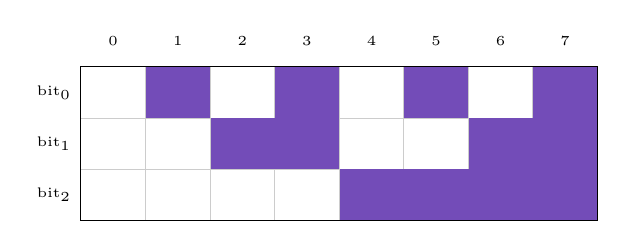
\begin{tikzpicture}[xscale=0.82, yscale=0.65]
    % Grid labels
    \foreach \x/\lbl in {0/0,1/1,2/2,3/3,4/4,5/5,6/6,7/7}
      \node[font=\tiny] at (\x+0.5, 3.5) {\lbl};

    % bit0 row
    \node[font=\tiny, left] at (0, 2.5) {bit$_0$};
    \foreach \x in {1,3,5,7}
      \fill[boIndigo!70] (\x, 2) rectangle (\x+1, 3);
    \foreach \x in {0,2,4,6}
      \draw[gray!40] (\x, 2) rectangle (\x+1, 3);

    % bit1 row
    \node[font=\tiny, left] at (0, 1.5) {bit$_1$};
    \foreach \x in {2,3,6,7}
      \fill[boIndigo!70] (\x, 1) rectangle (\x+1, 2);
    \foreach \x in {0,1,4,5}
      \draw[gray!40] (\x, 1) rectangle (\x+1, 2);

    % bit2 row
    \node[font=\tiny, left] at (0, 0.5) {bit$_2$};
    \foreach \x in {4,5,6,7}
      \fill[boIndigo!70] (\x, 0) rectangle (\x+1, 1);
    \foreach \x in {0,1,2,3}
      \draw[gray!40] (\x, 0) rectangle (\x+1, 1);

    % Outer frame
    \draw (0,0) rectangle (8,3);
  \end{tikzpicture}
  \end{center}

  \begin{block}{Key idea}
    Position can be encoded through signals that vary at \textbf{different frequencies}.
  \end{block}
\end{frame}
%
%..................................................................
%
\begin{frame}{Binary as Multiple Frequencies}
\begin{center}

\includegraphics[scale=.4]{../05-pictures/chapter-04_pic_3.png} 
\end{center}
\end{frame}
%
%..................................................................
%
\begin{frame}{Binary Solves Some Problems}

Binary has attractive properties.

\medskip

\begin{itemize}
    \item Codes are bounded: values are only 0 or 1.
    \item Positions can be uniquely identified.
    \item The same position has the same binary representation in any sequence.
    \item Different bits capture different positional scales.
\end{itemize}

\medskip

\begin{block}{Important insight}
Binary already contains the essential idea behind sinusoidal positional encoding:
\[
\text{use several frequencies to encode position.}
\]
\end{block}

\end{frame}
%
%..................................................................
%
\begin{frame}{But Binary Is Too Discontinuous}
\small
Binary has a serious problem.
\[
3 = 011,
\qquad
4 = 100.
\]

The position changes by one step, but all bits change.

\begin{alertblock}{Problem}
Nearby positions can have very different binary vectors.
\end{alertblock}

This is not ideal for neural networks, because neural networks rely on:

\begin{itemize}
    \item continuous representations;
    \item smooth transformations;
    \item gradients;
    \item dot products and distances.
\end{itemize}

\begin{block}{Transition}
Can we keep the multi-frequency structure of binary but make it smooth?
\end{block}

\end{frame}
%
%..................................................................
%
\begin{frame}{From Binary Bits to Smooth Waves}

Binary bits are hard oscillators:

\[
0,1,0,1,0,1,\ldots
\]

Sinusoids are smooth oscillators:

\[
\sin(\omega \cdot pos),
\qquad
\cos(\omega \cdot pos).
\]

\begin{columns}[T]

\column{0.48\textwidth}

\begin{block}{Binary}
\begin{itemize}
    \item discrete;
    \item discontinuous;
    \item abrupt bit flips;
    \item hard positional code.
\end{itemize}
\end{block}

\column{0.48\textwidth}

\begin{block}{Sinusoidal}
\begin{itemize}
    \item continuous;
    \item smooth;
    \item gradual variation;
    \item soft positional code.
\end{itemize}
\end{block}

\end{columns}

%\begin{alertblock}{Main intuition}
%Sinusoidal positional encoding is smooth binary counting.
%\end{alertblock}

\end{frame}
%
%..................................................................
%
\begin{frame}{What Does Frequency Mean?}

A sinusoidal positional signal has the form:
\[
pos \mapsto \sin(\omega \cdot pos).
\]

The frequency \(\omega\) determines how quickly the signal changes as position increases.

\begin{columns}[T]

\column{0.48\textwidth}

\begin{block}{High frequency}
\begin{itemize}
    \item changes quickly;
    \item distinguishes nearby positions;
    \item similar to low-order binary bits.
\end{itemize}
\end{block}

\column{0.48\textwidth}

\begin{block}{Low frequency}
\begin{itemize}
    \item changes slowly;
    \item captures broad location;
    \item similar to high-order binary bits.
\end{itemize}
\end{block}

\end{columns}

\begin{alertblock}{Clarification}
Frequency is not a property of a word.  
It is a property of the positional signal.
\end{alertblock}

\end{frame}
%
%..................................................................
%
\begin{frame}{The Transformer Formula}

The original Transformer uses:

\[
PE(pos,2i)
=
\sin
\left(
\frac{pos}{10000^{2i/d_{\text{model}}}}
\right),
\]

\[
PE(pos,2i+1)
=
\cos
\left(
\frac{pos}{10000^{2i/d_{\text{model}}}}
\right).
\]

\begin{block}{Meaning of the symbols}
\begin{itemize}
    \item \(pos\): token position;
    \item \(i\): index of the sine--cosine pair;
    \item \(d_{\text{model}}\): embedding dimension;
    \item even dimensions use sine;
    \item odd dimensions use cosine.
\end{itemize}
\end{block}

\end{frame}
%
%..................................................................
%
\begin{frame}{The Transformer Formula}
\begin{center}
\vspace{-.3cm}

\includegraphics[scale=.45]{../05-pictures/chapter-04_pic_4.png} 
\end{center}
\end{frame}
%
%..................................................................
%
\begin{frame}{Reading the Formula as Oscillators}
\small
Rewrite the formula as:

\[
PE(pos,2i)=\sin(\omega_i pos),
\]

\[
PE(pos,2i+1)=\cos(\omega_i pos),
\]

where

\[
\omega_i =
\frac{1}{10000^{2i/d_{\text{model}}}}.
\]

\begin{alertblock}{Interpretation}
Each sine--cosine pair is an oscillator running at frequency \(\omega_i\).
\end{alertblock}

As \(i\) increases, \(\omega_i\) decreases. Therefore:

\begin{itemize}
    \item early dimensions change quickly;
    \item later dimensions change slowly.
\end{itemize}

\end{frame}
%
%..................................................................
%
\begin{frame}{Why the Number 10000?}
\small
The constant \(10000\) controls the range of wavelengths. The denominator

\[
10000^{2i/d_{\text{model}}}
\]

creates a geometric progression across dimensions.

\begin{block}{Intuition}
The model receives positional clocks at many different scales.
\end{block}

This resembles binary:

\[
1,2,4,8,16,\ldots
\]

but uses smooth waves rather than abrupt bit flips.

\medskip

\begin{alertblock}{Important}
The exact constant is an engineering choice.  
The essential idea is the geometric spread of frequencies.
\end{alertblock}

\end{frame}
%
%..................................................................
%
\begin{frame}{A Small Example}

Suppose \(d_{\text{model}}=4\). Then:

\[
PE(pos)=
\left[
\sin(pos),
\cos(pos),
\sin\left(\frac{pos}{100}\right),
\cos\left(\frac{pos}{100}\right)
\right].
\]

\medskip

For the first few positions:

\[
\begin{array}{c|cccc}
pos & PE_0 & PE_1 & PE_2 & PE_3 \\
\hline
0 & 0.00 & 1.00 & 0.00 & 1.00 \\
1 & 0.84 & 0.54 & 0.01 & 1.00 \\
2 & 0.91 & -0.42 & 0.02 & 1.00 \\
3 & 0.14 & -0.99 & 0.03 & 1.00
\end{array}
\]

\medskip

\begin{block}{Reading the table}
The first pair changes quickly; the second pair changes slowly.
\end{block}

\end{frame}
%
%..................................................................
%
\begin{frame}{Adding the Encoding to the Token Embedding}
\small
The final input to the Transformer is:

\[
z_{pos}
=
e_{\text{token}(pos)}
+
PE(pos).
\]

\begin{exampleblock}{Example}
For the sentence \textbf{``the bank raised rates... ''}, the token ``bank'' at position 1 is represented as:
\[
z_1 = e_{\text{bank}} + PE(1).
\]
\end{exampleblock}

If the same word appears in another position:

\[
z_5 = e_{\text{bank}} + PE(5).
\]

\begin{alertblock}{Consequence}
The same word obtains different input representations at different positions.
\end{alertblock}

\end{frame}
%
%..................................................................
%
\begin{frame}{Why Sine and Cosine Together?}
\small
A Sine--Cosine Pair Is a Clock Hand. For one frequency \(\omega\), define:

\[
u_\omega(pos)
=
\begin{bmatrix}
\sin(\omega pos) \\
\cos(\omega pos)
\end{bmatrix}.
\]


This vector lies on the unit circle.


\begin{center}
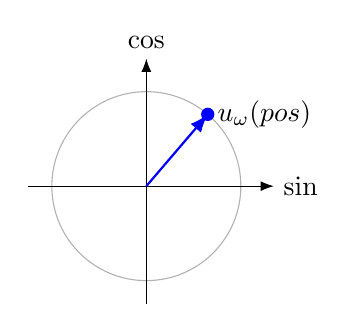
\begin{tikzpicture}[scale=1.2]
    \draw[gray!60] (0,0) circle (1);
    \draw[-{Latex}] (-1.25,0) -- (1.35,0) node[right] {$\sin$};
    \draw[-{Latex}] (0,-1.25) -- (0,1.35) node[above] {$\cos$};
    \draw[-{Latex}, thick, blue] (0,0) -- (0.65,0.76);
    \fill[blue] (0.65,0.76) circle (2pt);
    \node[right] at (0.65,0.76) {$u_\omega(pos)$};
\end{tikzpicture}
\end{center}

Increasing the position rotates the clock hand.

\end{frame}
%
%..................................................................
%
\begin{frame}{Relative Position as Rotation}

Moving from \(pos\) to \(pos+k\) rotates the sine--cosine pair.

\medskip

Using trigonometric identities:

\[
\sin(\omega(pos+k))
=
\sin(\omega pos)\cos(\omega k)
+
\cos(\omega pos)\sin(\omega k),
\]

\[
\cos(\omega(pos+k))
=
\cos(\omega pos)\cos(\omega k)
-
\sin(\omega pos)\sin(\omega k).
\]

\medskip

\begin{alertblock}{Key property}
For a fixed offset \(k\), the encoding at \(pos+k\) can be obtained from the encoding at \(pos\) through a linear transformation.
\end{alertblock}

\end{frame}
%
%..................................................................
%
\begin{frame}{The Rotation Matrix}

The previous identities can be written as:

\[
\begin{bmatrix}
\sin(\omega(pos+k)) \\
\cos(\omega(pos+k))
\end{bmatrix}
=
\begin{bmatrix}
\cos(\omega k) & \sin(\omega k) \\
-\sin(\omega k) & \cos(\omega k)
\end{bmatrix}
\begin{bmatrix}
\sin(\omega pos) \\
\cos(\omega pos)
\end{bmatrix}.
\]

\medskip

\begin{block}{Interpretation}
A relative shift in position corresponds to a rotation.
\end{block}

\medskip

\begin{alertblock}{Why this matters}
The transformation depends on the distance \(k\), not on the absolute position \(pos\).
\end{alertblock}

\end{frame}
%
%..................................................................
%
\begin{frame}{Dot Products Reveal Relative Distance}

For one sine--cosine clock:

\[
u_\omega(pos)
=
\begin{bmatrix}
\sin(\omega pos) \\
\cos(\omega pos)
\end{bmatrix}.
\]

The dot product between two positions is:

\[
u_\omega(pos)^\top u_\omega(pos+k)
=
\cos(\omega k).
\]

\medskip

\begin{alertblock}{Important consequence}
The similarity between two positional encodings depends on their relative distance.
\end{alertblock}

\medskip

Self-attention is based on dot products, so this property is especially useful.

\end{frame}
%__________________________________________________________________________
%
\section{The Transformer Architecture}
%__________________________________________________________________________
%
\begin{frame}{The Transformer: Overview (Vaswani et al., 2017)}
  \begin{columns}[c]
    \begin{column}{0.46\textwidth}
      The Transformer replaces recurrence entirely with attention. It consists of:

      \vspace{0.3em}
      \textbf{Encoder (left):} processes the full input bidirectionally.
      Each layer contains:
      \begin{enumerate}
        \item Multi-head self-attention
        \item Position-wise feed-forward network
        \item Residual connections + layer normalisation
      \end{enumerate}

      \vspace{0.3em}
      \textbf{Decoder (right):} generates output auto-regressively.
      Adds masked self-attention and cross-attention to encoder output.
    \end{column}
    \begin{column}{0.48\textwidth}
      \begin{center}
      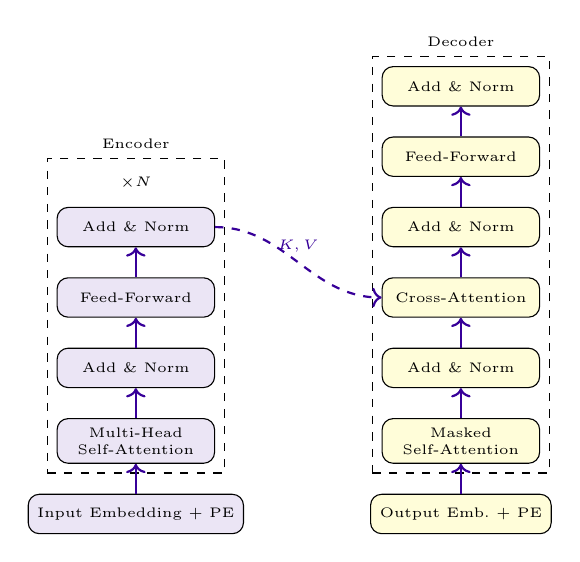
\begin{tikzpicture}[
        tblock/.style={draw, rounded corners, fill=bolight,
                       minimum width=2.0cm, minimum height=0.50cm,
                       font=\tiny, align=center},
        dblock/.style={draw, rounded corners, fill=yellow!15,
                       minimum width=2.0cm, minimum height=0.50cm,
                       font=\tiny, align=center},
        node distance=0.38cm
      ]
        % ── ENCODER ──
        \node[tblock] (E_emb)  {Input Embedding + PE};
        \node[tblock, above=of E_emb]  (E_att)  {Multi-Head\\Self-Attention};
        \node[tblock, above=of E_att]  (E_an1)  {Add \& Norm};
        \node[tblock, above=of E_an1]  (E_ff)   {Feed-Forward};
        \node[tblock, above=of E_ff]   (E_an2)  {Add \& Norm};
        \node[font=\tiny, above=0.1cm of E_an2] (EN) {$\times N$};
        \node[draw, dashed, fit=(E_att)(E_an1)(E_ff)(E_an2)(EN),
              label={[font=\tiny]above:Encoder}] (EBOX) {};

        \draw[arr] (E_emb) -- (E_att);
        \draw[arr] (E_att) -- (E_an1);
        \draw[arr] (E_an1) -- (E_ff);
        \draw[arr] (E_ff)  -- (E_an2);

        % ── DECODER ──
        \node[dblock, right=1.6cm of E_emb] (D_emb) {Output Emb.\ + PE};
        \node[dblock, above=of D_emb]  (D_mask) {Masked\\Self-Attention};
        \node[dblock, above=of D_mask] (D_an1)  {Add \& Norm};
        \node[dblock, above=of D_an1]  (D_cross) {Cross-Attention};
        \node[dblock, above=of D_cross] (D_an2)  {Add \& Norm};
        \node[dblock, above=of D_an2]  (D_ff)   {Feed-Forward};
        \node[dblock, above=of D_ff]   (D_an3)  {Add \& Norm};
        \node[draw, dashed, fit=(D_mask)(D_an1)(D_cross)(D_an2)(D_ff)(D_an3),
              label={[font=\tiny]above:Decoder}] (DBOX) {};

        \draw[arr] (D_emb)  -- (D_mask);
        \draw[arr] (D_mask) -- (D_an1);
        \draw[arr] (D_an1)  -- (D_cross);
        \draw[arr] (D_cross)-- (D_an2);
        \draw[arr] (D_an2)  -- (D_ff);
        \draw[arr] (D_ff)   -- (D_an3);

        % Cross-attention connection from encoder
        \draw[arr, dashed]
          (E_an2.east) to[out=0,in=180]
          node[above,font=\tiny]{$K,V$} (D_cross.west);
      \end{tikzpicture}
      \end{center}
    \end{column}
  \end{columns}
\end{frame}
%
%..................................................................
%
\begin{frame}{One Encoder Block: Data Flow and Dimensions}

\begin{columns}[T]

%% --- Left column: TikZ diagram ---
\begin{column}{0.44\textwidth}
\centering
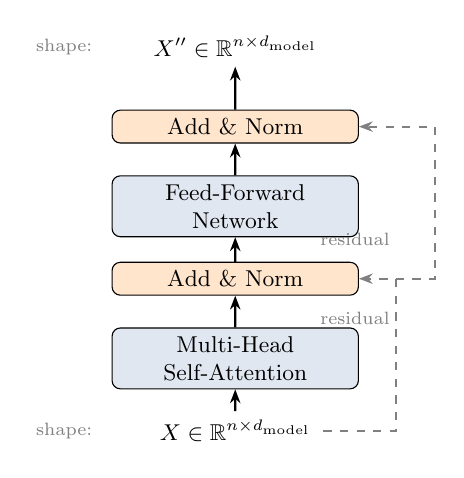
\begin{tikzpicture}[
  box/.style={
    draw, rounded corners=3pt, fill=uniboblue!12,
    minimum width=3.4cm, minimum height=0.55cm,
    font=\small, align=center},
  norm/.style={
    draw, rounded corners=3pt, fill=orange!20,
    minimum width=3.4cm, minimum height=0.45cm,
    font=\small, align=center},
  arr/.style={-{Stealth[length=5pt]}, thick},
  res/.style={-{Stealth[length=5pt]}, thick, dashed, gray},
  lbl/.style={font=\scriptsize, gray},
  scale=0.92, every node/.style={transform shape}
]

%% Nodes (bottom to top to follow paper convention)
\node[box] (mha)  at (0, 0)    {Multi-Head\\Self-Attention};
\node[norm] (an1) at (0, 1.10) {Add \& Norm};
\node[box]  (ffn) at (0, 2.10) {Feed-Forward\\Network};
\node[norm] (an2) at (0, 3.20) {Add \& Norm};

%% Input / Output labels
\node[font=\small] (inp) at (0, -1.0) {%
  $X \in \mathbb{R}^{n \times \dmodel}$};
\node[font=\small] (out) at (0,  4.3) {%
  $X'' \in \mathbb{R}^{n \times \dmodel}$};

%% Main flow arrows
\draw[arr] (inp) -- (mha);
\draw[arr] (mha) -- (an1);
\draw[arr] (an1) -- (ffn);
\draw[arr] (ffn) -- (an2);
\draw[arr] (an2) -- (out);

%% First residual connection (around MHA)
\draw[res]
  (inp.east) ++( 0.05,0)
    -| ++(1.0, 0)
    |- (an1.east);
\node[lbl, anchor=west] at (1.05, 0.55) {residual};

%% Second residual connection (around FFN)
\draw[res]
  (an1.east) ++(0.05,0)
    -| ++(1.0, 0)
    |- (an2.east);
\node[lbl, anchor=west] at (1.05, 1.65) {residual};

%% Dimension annotations
\node[lbl, anchor=east] at (-1.85, -1.0) {shape:};
\node[lbl, anchor=east] at (-1.85,  4.3) {shape:};

\end{tikzpicture}
\end{column}

%% --- Right column: explanations ---
\begin{column}{0.54\textwidth}
\small
Every encoder block applies four operations in sequence:

\medskip
\begin{enumerate}\itemsep4pt
  \item \textbf{Multi-head self-attention}\\
    Each token attends to every other token.\\
    Input and output both live in
    $\mathbb{R}^{n \times \dmodel}$.

  \item \textbf{Add \& Norm} (first)\\
    The input $X$ is added to the attention output
    (residual connection), then Layer\-Norm is applied
    token-wise: $X' = \mathrm{LN}(X + \widetilde{X})$.

  \item \textbf{Position-wise feed-forward network}\\
    The same two-layer MLP is applied to each of the $n$
    token vectors independently.

  \item \textbf{Add \& Norm} (second)\\
    $X'' = \mathrm{LN}(X' + \mathrm{FFN}(X'))$.
\end{enumerate}

\medskip
\begin{alertblock}{Dimension invariance}
Input and output have the \emph{same} shape
$n \times \dmodel$. Blocks can therefore be
stacked freely.
\end{alertblock}
\end{column}

\end{columns}
\end{frame}
%
%..................................................................
%
\begin{frame}{Stacking $N$ Encoder Blocks: What Depth Achieves}
\small
\begin{columns}[T]
\begin{column}{0.52\textwidth}

\textbf{Architecture}: the output of block $\ell$ is the input of block $\ell+1$:
\[
  X^{(\ell)} = \mathrm{EncoderBlock}\!\left(X^{(\ell-1)}\right),
  \quad \ell = 1, \ldots, N.
\]
All blocks share the \emph{same structure} but have
\emph{independent, learned parameters}.

\textbf{What successive layers tend to capture:}

\begin{tabular}{@{}cl@{}}
  \toprule
  Layers & Representation content \\
  \midrule
  Early   & Surface form, local syntax,\\
           & morphology \\[2pt]
  Middle  & Phrase structure, entity type,\\
           & coreference \\[2pt]
  Late    & Semantic roles, long-range\\
           & dependencies, task cues \\
  \bottomrule
\end{tabular}

%\smallskip
%\footnotesize(Evidence from probing studies on BERT; Tenney et al.\ 2019.)
\end{column}
\begin{column}{0.44\textwidth}
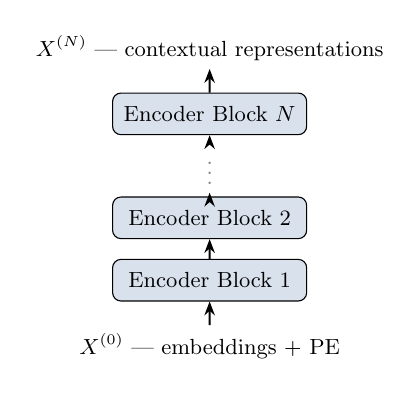
\begin{tikzpicture}[
  blk/.style={draw, fill=uniboblue!15, rounded corners=3pt,
              minimum width=2.8cm, minimum height=0.6cm,
              font=\small, align=center},
  arr/.style={-{Stealth[length=5pt]}, thick},
  scale=0.88, every node/.style={transform shape}
]

\node[font=\small] (x0) at (0,0) {$X^{(0)}$ — embeddings + PE};
\node[blk] (b1) at (0, 0.95) {Encoder Block 1};
\node[blk] (b2) at (0, 1.85) {Encoder Block 2};
\node[font=\small, gray] (dots) at (0, 2.60) {$\vdots$};
\node[blk] (bN) at (0, 3.35) {Encoder Block $N$};
\node[font=\small] (xN) at (0, 4.30) {$X^{(N)}$ — contextual representations};

\draw[arr] (x0)   -- (b1);
\draw[arr] (b1)   -- (b2);
\draw[arr] (b2)   -- (dots);
\draw[arr] (dots) -- (bN);
\draw[arr] (bN)   -- (xN);

\end{tikzpicture}

\begin{block}{Analogy}
  Stacking Transformer blocks resembles
  stacking convolutional layers in a CNN:
  each layer sees a progressively richer,
  more global view of the input.
\end{block}

\end{column}
\end{columns}

\end{frame}
%
%..................................................................
%
\begin{frame}{Residual Connections and Layer Normalisation}
  Every sub-layer (attention or feed-forward) is wrapped in:
  \[
    \mathrm{output} = \mathrm{LayerNorm}\!\bigl(x + \mathrm{SubLayer}(x)\bigr).
  \]

  \begin{columns}[t]
    \begin{column}{0.44\textwidth}
      \begin{block}{Residual connections (He et al., 2016)}
        \begin{itemize}
          \item Allow gradients to flow directly through the network via the identity
                shortcut.
          \item Enable training of very deep models: 6, 12, 24, 96+ layers.
          \item Without them, deep Transformers simply do not converge.
        \end{itemize}
      \end{block}
    \end{column}
    \begin{column}{0.50\textwidth}
      \begin{block}{Layer normalisation (Ba et al., 2016)}
        \begin{itemize}
          \item Normalises activations across features, not across the batch unlike
                BatchNorm.
          \item Stabilises training and reduces sensitivity to learning rate.
          \item Applied per-token, per-layer.
        \end{itemize}
      \end{block}
    \end{column}
  \end{columns}
\end{frame}
%
%..................................................................
%
\begin{frame}{Residual Connections – Why They Work}
  \begin{columns}[c]
    \begin{column}{0.44\textwidth}
      \begin{block}{Without residual}
        \centering\vspace{0.3em}
        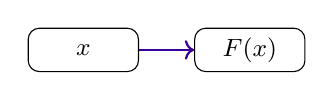
\begin{tikzpicture}[node distance=0.6cm]
          \node[sblock] (x) {$x$};
          \node[sblock, right=0.7cm of x] (f) {$F(x)$};
          \draw[arr] (x) -- (f);
        \end{tikzpicture}\\[0.3em]
        {\small Gradient must flow through every layer.}
        \vspace{0.3em}
      \end{block}
    \end{column}
    \begin{column}{0.50\textwidth}
      \begin{block}{With residual}
        \centering\vspace{0.3em}
        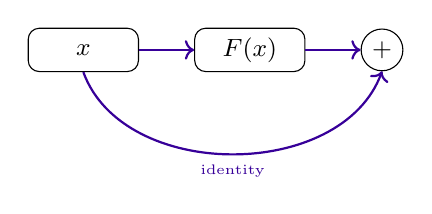
\begin{tikzpicture}[node distance=0.6cm]
          \node[sblock] (x) {$x$};
          \node[sblock, right=0.7cm of x] (f) {$F(x)$};
          \node[draw, circle, right=0.7cm of f, inner sep=2pt, font=\small] (plus)
               {$+$};
          \draw[arr] (x) -- (f);
          \draw[arr] (f) -- (plus);
          \draw[arr] (x.south) to[out=-70,in=-110] node[below,font=\tiny]{identity}
               (plus.south);
        \end{tikzpicture}\\[0.3em]
        {\small Gradient has a direct path $\to$ deep networks can train.}
        \vspace{0.3em}
      \end{block}
    \end{column}
  \end{columns}

  \vspace{0.6em}
  The gradient of the output with respect to the input includes a term that is exactly
  $\mathbf{I}$ (the identity), regardless of what $F$ does.  This prevents gradient
  vanishing even with 96+ layers.
\end{frame}
%
%..................................................................
%
\begin{frame}{Why a Feed-Forward Layer after Self-Attention?}
  Self-attention allows each token to collect information from the other tokens in the
  sequence:
  \[
    x_i \;\longrightarrow\; \tilde{x}_i,
  \]
  where $\tilde{x}_i$ is a contextualized representation of token $i$.

  \vspace{0.4em}
  However, attention mainly performs a \emph{content-dependent mixing} of token
  representations.

  After this mixing step, the model still needs a mechanism to transform each
  contextualized vector into a richer feature representation.

  \vspace{0.4em}
  \begin{block}{Key idea}
    Self-attention decides \emph{which} tokens interact; the feed-forward layer decides
    \emph{how} each resulting token representation is transformed.
  \end{block}
\end{frame}
%
%..................................................................
%
\begin{frame}{The Position-Wise Feed-Forward Network}
  In each Transformer block, the feed-forward sublayer is applied independently to
  each token position:
  \[
    \mathrm{FFN}(x_i) = W_2\,\sigma(W_1 x_i + b_1) + b_2,
    \quad i = 1, \ldots, n.
  \]
  The same function is reused for all positions:
  \[
    \mathrm{FFN}(x_1),\;\mathrm{FFN}(x_2),\;\ldots,\;\mathrm{FFN}(x_n).
  \]
  If the input sequence is represented as a matrix
  $X \in \mathbb{R}^{n \times d_{\mathrm{model}}}$,
  then the feed-forward layer maps
  \[
    X \;\longrightarrow\; \mathrm{FFN}(X) \in \mathbb{R}^{n \times d_{\mathrm{model}}}.
  \]
\end{frame}
%
%..................................................................
%
\begin{frame}{Why Two Linear Layers?}
  The Transformer feed-forward sublayer is usually a two-layer neural network:
  \[
    \mathrm{FFN}(x_i) = W_2\,\sigma(W_1 x_i + b_1) + b_2.
  \]
  The first projection \textbf{expands} the representation:
  \[
    W_1: \mathbb{R}^{d_{\mathrm{model}}} \to \mathbb{R}^{d_{\mathrm{ff}}}.
  \]
  The second projection maps it \textbf{back} to the model dimension:
  \[
    W_2: \mathbb{R}^{d_{\mathrm{ff}}} \to \mathbb{R}^{d_{\mathrm{model}}}.
  \]
  Typically, $d_{\mathrm{ff}} > d_{\mathrm{model}}$.
\end{frame}
%
%..................................................................
%
\begin{frame}{Why Two Linear Layers?}
  \begin{block}{Interpretation}
    The expansion creates a higher-dimensional feature space; the non-linearity allows
    richer transformations; the final projection restores the dimension needed by the
    next Transformer block.
  \end{block}
\end{frame}
%
%..................................................................
%
\begin{frame}{Self-Attention and Feed-Forward Layers Play Different Roles}
  \begin{columns}[t]
    \begin{column}{0.44\textwidth}
      \begin{block}{Self-attention}
        \centering\vspace{0.3em}
        $\displaystyle\mathrm{Attention}(Q,K,V)
          = \mathrm{softmax}\!\!\left(\!\frac{QK^\top}{\sqrt{d_k}}\!\right)V$
        \vspace{0.3em}
        \begin{itemize}
          \item mixes information across tokens;
          \item builds context-dependent representations;
          \item captures relations such as syntactic or semantic dependencies.
        \end{itemize}
      \end{block}
    \end{column}
    \begin{column}{0.50\textwidth}
      \begin{block}{Feed-forward network}
        \centering\vspace{0.3em}
        $\mathrm{FFN}(x_i) = W_2\,\sigma(W_1 x_i + b_1) + b_2$
        \vspace{0.3em}
        \begin{itemize}
          \item acts independently on each token;
          \item introduces non-linear feature transformation;
          \item refines the contextual representation produced by attention.
        \end{itemize}
      \end{block}
    \end{column}
  \end{columns}
\end{frame}
%
%..................................................................
%
\begin{frame}{The Original Transformer: Key Hyperparameters}
\small
Vaswani et al.\ (2017) trained two model sizes on the WMT 2014 translation task.
Understanding these numbers anchors the later discussion of scaling.

\bigskip
\begin{center}
\renewcommand{\arraystretch}{1.25}
\begin{tabular}{@{}lcc@{}}
  \toprule
  \textbf{Hyperparameter} & \textbf{Base model} & \textbf{Large model} \\
  \midrule
  Encoder/decoder layers $N$    & 6      & 6      \\
  Model dimension $\dmodel$     & 512    & 1\,024 \\
  Feed-forward dimension $\dff$ & 2\,048 & 4\,096 \\
  Number of heads $h$           & 8      & 16     \\
  Head dimension $\dk = \dv$    & 64     & 64     \\
  \midrule
  Trainable parameters          & $\approx$ 65\,M  & $\approx$ 213\,M \\
  Training steps                & 100\,K & 300\,K \\
  \midrule
  BLEU (EN$\to$DE)              & 27.3   & 28.4   \\
  \bottomrule
\end{tabular}
\end{center}
\end{frame}
%
%..................................................................
%
\begin{frame}{The Original Transformer: Key Hyperparameters}
\begin{columns}[T]
\begin{column}{0.48\textwidth}
\begin{block}{Note on head dimension}
  $\dk = \dmodel / h$:
  each head operates in a \emph{lower}-dimensional space,
  so the total cost of multi-head attention is comparable
  to single-head attention at full dimension.
\end{block}
\end{column}
\begin{column}{0.48\textwidth}
\begin{alertblock}{Perspective}
  65\,M parameters was state-of-the-art in 2017.
  Contemporary LLMs range from 7\,B (LLaMA 3.1 8B)
  to hundreds of billions of parameters—
  the architecture is the same; the scale is not.
\end{alertblock}
\end{column}
\end{columns}

\end{frame}
%
%..................................................................
%
\begin{frame}{Masked Self-Attention: Enabling Auto-regressive Generation}
  In the decoder, the model generates tokens one at a time, left to right.  During
  training, it must not see future tokens – this would be ``cheating''.

  \vspace{0.3em}
  Solution: apply a mask to the attention score matrix before softmax:
  \[
    S'_{ij} =
    \begin{cases}
      \dfrac{q_i^\top k_j}{\sqrt{d_k}} & \text{if } j \le i,\\[6pt]
      -\infty & \text{if } j > i.
    \end{cases}
  \]
  After softmax, $-\infty$ entries become 0 – future positions are invisible.

  \vspace{0.3em}
  \begin{columns}[c]
    \begin{column}{0.42\textwidth}
      \begin{center}
      \small$
      \begin{pmatrix}
        s_{11} & -\infty & -\infty & -\infty \\
        s_{21} & s_{22}  & -\infty & -\infty \\
        s_{31} & s_{32}  & s_{33}  & -\infty \\
        s_{41} & s_{42}  & s_{43}  & s_{44}
      \end{pmatrix}
      $
      \end{center}
    \end{column}
    \begin{column}{0.52\textwidth}
      Causal mask: each token can only attend to itself and to previous tokens.

      \vspace{0.3em}
      This is what makes GPT-style models auto-regressive: position $i$ only ``sees''
      positions $1, \ldots, i$.
    \end{column}
  \end{columns}
\end{frame}
%
%..................................................................
%
\begin{frame}{The Full Decoder Block: Three Sub-Layers}

\begin{columns}[T]

%% --- Left column: diagram ---
\begin{column}{0.42\textwidth}
\centering
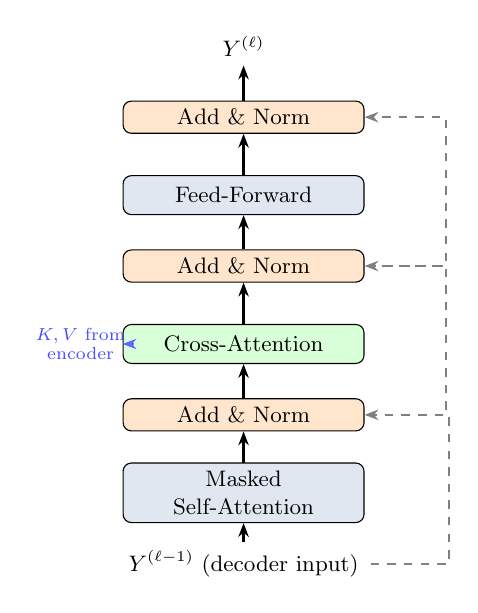
\begin{tikzpicture}[
  box/.style={
    draw, rounded corners=3pt, fill=uniboblue!12,
    minimum width=3.4cm, minimum height=0.55cm,
    font=\small, align=center},
  norm/.style={
    draw, rounded corners=3pt, fill=orange!20,
    minimum width=3.4cm, minimum height=0.45cm,
    font=\small, align=center},
  cbox/.style={
    draw, rounded corners=3pt, fill=green!15,
    minimum width=3.4cm, minimum height=0.55cm,
    font=\small, align=center},
  arr/.style={-{Stealth[length=5pt]}, thick},
  res/.style={-{Stealth[length=5pt]}, thick, dashed, gray},
  kv/.style={-{Stealth[length=5pt]}, thick, blue!60},
  lbl/.style={font=\scriptsize, gray},
  scale=0.90, every node/.style={transform shape}
]

\node[font=\small]  (inp) at (0,-1.0) {$Y^{(\ell-1)}$ (decoder input)};
\node[box]          (msa) at (0, 0.0) {Masked\\Self-Attention};
\node[norm]         (an1) at (0, 1.1) {Add \& Norm};
\node[cbox]         (ca)  at (0, 2.1) {Cross-Attention};
\node[norm]         (an2) at (0, 3.2) {Add \& Norm};
\node[box]          (ffn) at (0, 4.2) {Feed-Forward};
\node[norm]         (an3) at (0, 5.3) {Add \& Norm};
\node[font=\small]  (out) at (0, 6.3) {$Y^{(\ell)}$};

\draw[arr] (inp) -- (msa);
\draw[arr] (msa) -- (an1);
\draw[arr] (an1) -- (ca);
\draw[arr] (ca)  -- (an2);
\draw[arr] (an2) -- (ffn);
\draw[arr] (ffn) -- (an3);
\draw[arr] (an3) -- (out);

%% Residual 1
\draw[res] (inp.east)++(0.05,0) -| ++(1.1,0) |- (an1.east);
%% Residual 2
\draw[res] (an1.east)++(0.05,0) -| ++(1.1,0) |- (an2.east);
%% Residual 3
\draw[res] (an2.east)++(0.05,0) -| ++(1.1,0) |- (an3.east);

%% K,V from encoder
\node[font=\scriptsize, blue!70, align=center] (enc) at (-2.3, 2.1) {$K,V$ from\\encoder};

\draw[kv] (enc) -- (ca.west);

\end{tikzpicture}
\end{column}

%% --- Right column: descriptions ---
\begin{column}{0.55\textwidth}
\small
The decoder block has \textbf{three} sub-layers
(vs.\ two in the encoder).

\medskip
\textbf{\textsf{Sub-layer 1 — Masked self-attention}}\\
The decoder attends to its own previously generated
tokens. The causal mask prevents attending to
future positions.
\[
  Q = K = V = Y^{(\ell-1)},\quad
  \text{mask: } j \le i \text{ only.}
\]

\medskip
\textbf{\textsf{Sub-layer 2 — Cross-attention}}\\
Queries come from the decoder; keys and values come
from the encoder's final output $X^{(N)}$.
This is how the decoder reads the source sequence.
\[
  Q = Y W^Q,\quad K = X^{(N)}W^K,\quad V = X^{(N)}W^V.
\]

\end{column}
\end{columns}

\end{frame}
%
%..................................................................
%
\begin{frame}{The Full Decoder Block: Three Sub-Layers}

\begin{columns}[T]

%% --- Left column: diagram ---
\begin{column}{0.42\textwidth}
\centering
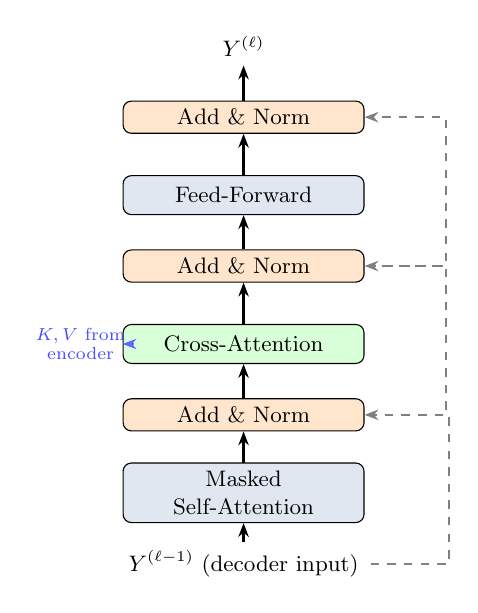
\begin{tikzpicture}[
  box/.style={
    draw, rounded corners=3pt, fill=uniboblue!12,
    minimum width=3.4cm, minimum height=0.55cm,
    font=\small, align=center},
  norm/.style={
    draw, rounded corners=3pt, fill=orange!20,
    minimum width=3.4cm, minimum height=0.45cm,
    font=\small, align=center},
  cbox/.style={
    draw, rounded corners=3pt, fill=green!15,
    minimum width=3.4cm, minimum height=0.55cm,
    font=\small, align=center},
  arr/.style={-{Stealth[length=5pt]}, thick},
  res/.style={-{Stealth[length=5pt]}, thick, dashed, gray},
  kv/.style={-{Stealth[length=5pt]}, thick, blue!60},
  lbl/.style={font=\scriptsize, gray},
  scale=0.90, every node/.style={transform shape}
]

\node[font=\small]  (inp) at (0,-1.0) {$Y^{(\ell-1)}$ (decoder input)};
\node[box]          (msa) at (0, 0.0) {Masked\\Self-Attention};
\node[norm]         (an1) at (0, 1.1) {Add \& Norm};
\node[cbox]         (ca)  at (0, 2.1) {Cross-Attention};
\node[norm]         (an2) at (0, 3.2) {Add \& Norm};
\node[box]          (ffn) at (0, 4.2) {Feed-Forward};
\node[norm]         (an3) at (0, 5.3) {Add \& Norm};
\node[font=\small]  (out) at (0, 6.3) {$Y^{(\ell)}$};

\draw[arr] (inp) -- (msa);
\draw[arr] (msa) -- (an1);
\draw[arr] (an1) -- (ca);
\draw[arr] (ca)  -- (an2);
\draw[arr] (an2) -- (ffn);
\draw[arr] (ffn) -- (an3);
\draw[arr] (an3) -- (out);

%% Residual 1
\draw[res] (inp.east)++(0.05,0) -| ++(1.1,0) |- (an1.east);
%% Residual 2
\draw[res] (an1.east)++(0.05,0) -| ++(1.1,0) |- (an2.east);
%% Residual 3
\draw[res] (an2.east)++(0.05,0) -| ++(1.1,0) |- (an3.east);

%% K,V from encoder
\node[font=\scriptsize, blue!70, align=center] (enc) at (-2.3, 2.1) {$K,V$ from\\encoder};

\draw[kv] (enc) -- (ca.west);

\end{tikzpicture}
\end{column}

%% --- Right column: descriptions ---
\begin{column}{0.55\textwidth}
\small
\medskip
\textbf{\textsf{Sub-layer 3 — Feed-forward network}}\\
Identical to the encoder FFN; applied position-wise.

\medskip
\begin{alertblock}{Decoder-only models}
GPT, LLaMA, Claude, Mistral: \textbf{no encoder, no
cross-attention}. Sub-layer~2 is removed entirely.
The model reads and generates within a single
masked-self-attention + FFN stack.
\end{alertblock}

\end{column}
\end{columns}

\end{frame}
%
%..................................................................
%
\begin{frame}{Cross-Attention: Connecting Encoder and Decoder}
  In the original encoder-decoder Transformer used for translation and summarisation:
  \begin{itemize}
    \item The encoder processes the input sequence and produces contextual
          representations.
    \item The decoder generates the output sequence one token at a time.
    \item Cross-attention lets the decoder ``look at'' the encoder's output:
  \end{itemize}
  \medskip
  \[
    Q = H_{\mathrm{decoder}}\,W^Q,
    \qquad
    K = H_{\mathrm{encoder}}\,W^K,
    \qquad
    V = H_{\mathrm{encoder}}\,W^V.
  \]
  \medskip
  Queries come from the decoder; keys and values come from the encoder.
\end{frame}
%
%..................................................................
%
\begin{frame}{Cross-Attention: Connecting Encoder and Decoder}
  \begin{block}{Modern landscape}
    Most current LLMs such as GPT-style, Claude-style, LLaMA-style and Mistral-style
    models are \textbf{decoder-only} – they do not have an encoder or cross-attention.
    The entire architecture is masked self-attention + FFN, repeated $N$ times.

    \vspace{0.3em}
    Encoder-decoder models such as T5 and BART are still used for specific tasks like
    summarisation and translation.
  \end{block}
\end{frame}
%
%..................................................................
%
\begin{frame}{Why ``Attention Is All You Need''?}
  \begin{center}
  {\small
  \begin{tabular}{lccc}
    \toprule
    & \textbf{RNN / LSTM} & \textbf{CNN} & \textbf{Transformer} \\
    \midrule
    Sequential operations  & $\mathcal{O}(n)$         & $\mathcal{O}(1)$         & $\mathcal{O}(1)$ \\
    Maximum path length    & $\mathcal{O}(n)$         & $\mathcal{O}(\log n)$    & $\mathcal{O}(1)$ \\
    Parallelisable?        & No                       & Yes                      & Yes \\
    Complexity / layer     & $\mathcal{O}(n\cdot d^2)$ & $\mathcal{O}(k\cdot n\cdot d^2)$ & $\mathcal{O}(n^2\cdot d)$ \\
    \bottomrule
  \end{tabular}}
  \end{center}

  \vspace{0.5em}
  The Transformer connects any two positions in the sequence with a single computation
  step (path length $\mathcal{O}(1)$), while being fully parallelisable on modern
  hardware such as GPUs and TPUs.
\end{frame}









%__________________________________________________________________________
%
\section{From the Transformer to Specialised Architectures}
%__________________________________________________________________________
%
\begin{frame}[plain]
  \vfill
  \begin{beamercolorbox}[sep=12pt,center,rounded=true,shadow=true]{title}
    \usebeamerfont{title}%
    From the Transformer\\to Specialised Architectures
  \end{beamercolorbox}
  \vfill
\end{frame}
%
%..................................................................
%
\begin{frame}{The Original Task: Sequence-to-Sequence}

The Transformer was introduced in \emph{Attention Is All You Need}
(Vaswani et al., 2017) to solve \textbf{machine translation}.

\medskip
\begin{block}{The core challenge}
  Given a source sentence of length $n$, produce a target sentence
  of length $m$, where $n \neq m$ in general.\\[4pt]
  \textbf{Example:} \quad
  \textit{``The Fed raised rates''} \;($n{=}4$)
  $\;\longrightarrow\;$
  \textit{``La Fed ha alzato i tassi''} \;($m{=}6$)
\end{block}

\medskip
This single task actually hides \textbf{two distinct sub-problems}:

\begin{enumerate}
  \item \textbf{Understanding the source:} build a rich internal
        representation that captures meaning, context, and
        long-range dependencies.
  \item \textbf{Generating the target:} produce tokens
        \emph{one at a time}, each conditioned on all tokens
        already generated \emph{and} on the source representation.
\end{enumerate}
\end{frame}
%
%..................................................................
%
\begin{frame}{The Original Task: Sequence-to-Sequence}
\begin{alertblock}{Key insight}
  The Transformer solves these two sub-problems with \textbf{two
  structurally different components}: the \textbf{encoder} and the
  \textbf{decoder}.
\end{alertblock}

\end{frame}
%
%..................................................................
%
\begin{frame}{Two Roles Within One Architecture}
\vspace{-1mm}
\begin{columns}[T]
  \begin{column}{0.47\textwidth}
    \begin{block}{The Encoder}
      \begin{itemize}\setlength\itemsep{0pt}\small
        \item Reads the \textbf{entire} source in parallel.
        \item $N$ layers of self-attention $+$ feed-forward.
        \item Output: $\mathbf{Z}\in\mathbb{R}^{n\times d}$, one
              contextual embedding per token.
        \item All positions attend freely to each other.
      \end{itemize}
      \vspace{2pt}\small\textbf{Role:} build a \emph{memory} of the source.
    \end{block}
  \end{column}

  \begin{column}{0.47\textwidth}
    \begin{block}{The Decoder}
      \begin{itemize}\setlength\itemsep{0pt}\small
        \item Generates the target \textbf{one token at a time}.
        \item \emph{Masked} self-attention: pos.\ $t$ only attends
              to $1,\ldots,t{-}1$.
        \item Reads encoder memory via \textbf{cross-attention}.
        \item Outputs a probability over the vocabulary.
      \end{itemize}
      \vspace{2pt}\small\textbf{Role:} generate conditioned on the memory.
    \end{block}
  \end{column}
\end{columns}

\vspace{2mm}
\begin{columns}[c]
  \begin{column}{0.55\textwidth}
    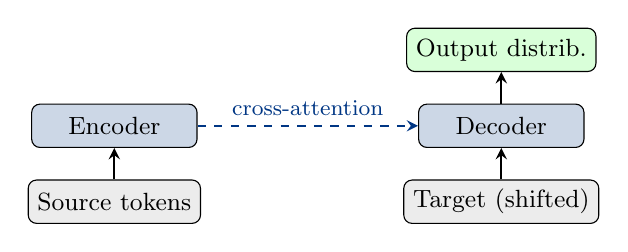
\begin{tikzpicture}[
        box/.style={draw, rounded corners=3pt, minimum width=2.1cm,
                    minimum height=0.55cm, align=center, font=\small},
        arr/.style={->, thick, >=stealth},
        cross/.style={->, thick, >=stealth, dashed, color=uniboblue}
      ]
      \node[box, fill=uniboblue!20] (enc) {Encoder};
      \node[box, fill=uniboblue!20, right=2.8cm of enc] (dec) {Decoder};
      \node[box, fill=gray!15, below=0.4cm of enc] (src) {Source tokens};
      \node[box, fill=gray!15, below=0.4cm of dec] (tgt) {Target (shifted)};
      \node[box, fill=green!15, above=0.4cm of dec] (out) {Output distrib.};
      \draw[arr] (src) -- (enc);
      \draw[arr] (tgt) -- (dec);
      \draw[arr] (dec) -- (out);
      \draw[cross] (enc) --
            node[above, font=\footnotesize]{cross-attention} (dec);
    \end{tikzpicture}
  \end{column}

  \begin{column}{0.42\textwidth}
    \begin{alertblock}{Key observation}
      \small Cross-attention is the \emph{only} coupling between
      encoder and decoder.  Remove it and the two components
      become \textbf{fully independent}.
    \end{alertblock}
  \end{column}
\end{columns}

\end{frame}
%
%..................................................................
%
\begin{frame}{Cross-Attention: The Bridge Between Encoder and Decoder}

Inside every decoder layer there is a \textbf{cross-attention}
sub-layer in addition to the usual masked self-attention.

\medskip
\begin{block}{Cross-attention formula}
  \[
    \text{CrossAttn}(Q_{\mathrm{dec}},\, K_{\mathrm{enc}},\, V_{\mathrm{enc}})
    \;=\;
    \operatorname{softmax}\!\left(\frac{Q_{\mathrm{dec}}\,K_{\mathrm{enc}}^\top}
    {\sqrt{d_k}}\right) V_{\mathrm{enc}}
  \]
  \begin{itemize}
    \item \textbf{Queries} $Q_{\mathrm{dec}}$: from the decoder's hidden
          states at the current generation step.
    \item \textbf{Keys and Values} $K_{\mathrm{enc}}, V_{\mathrm{enc}}$:
          from the encoder output $\mathbf{Z}$ --- computed once,
          reused at every decoder step.
  \end{itemize}
\end{block}
\end{frame}
%
%..................................................................
%
\begin{frame}{Cross-Attention: The Bridge Between Encoder and Decoder}
\begin{exampleblock}{Intuition}
  At each step the decoder \emph{asks a question} (query) about what
  it needs next, and the encoder \emph{answers} by highlighting the
  most relevant source tokens.  This mirrors how a human translator
  alternates between reading the original and writing the translation.
\end{exampleblock}

\medskip
\begin{alertblock}{Structural observation}
  Cross-attention is the \emph{only} information pathway between encoder
  and decoder.  Remove it and the two components become fully independent
  --- each exploitable on its own.
\end{alertblock}

\end{frame}
%
%..................................................................
%
\begin{frame}{A Key Observation: Two Independent Capabilities}

Once we recognise what each component does \emph{on its own},
a natural question arises: do we always need both?

\medskip
\begin{block}{The two standalone capabilities}
  \begin{itemize}
    \item The \textbf{encoder alone} produces rich contextual
          representations of any text --- no generation involved.
    \item The \textbf{decoder alone} can generate text
          autoregressively from a conditioning prefix --- no external
          memory needed.
    \item The coupling via cross-attention is \textbf{task-specific},
          not architecturally mandatory.
  \end{itemize}
\end{block}
\end{frame}
%
%..................................................................
%
\begin{frame}{A Key Observation: Two Independent Capabilities}
\begin{exampleblock}{Two research trajectories}
  \begin{description}
    \item[\textbf{Encoder only}]
          Maximise representation quality for \emph{understanding}
          tasks: classification, named-entity recognition,
          semantic similarity, retrieval.
    \item[\textbf{Decoder only}]
          Maximise generation quality for \emph{production}
          tasks: summarisation, dialogue, code generation,
          question answering.
  \end{description}
\end{exampleblock}

\medskip
These two paths produced two landmark families:
\textbf{BERT} (encoder only) and \textbf{GPT / modern LLMs}
(decoder only).

\end{frame}
%
%..................................................................
%
\begin{frame}{Encoder-Only Models: BERT}

\textbf{BERT} (Devlin et al., 2018) --- \emph{Bidirectional Encoder
Representations from Transformers} --- is a pure encoder stack
trained on two self-supervised objectives.

\begin{columns}[T]
  \begin{column}{0.47\textwidth}
    \begin{block}{Architecture}
      \begin{itemize}
        \item Encoder stack only; no decoder, no cross-attention.
        \item All tokens attend to \textbf{all other tokens} in
              both directions (\emph{bidirectional}).
        \item Output: one contextual embedding
              $\mathbf{z}_i \in \mathbb{R}^d$ per input token.
      \end{itemize}
    \end{block}
  \end{column}

  \begin{column}{0.47\textwidth}
    \begin{block}{Pre-training objectives}
      \begin{enumerate}
        \item \textbf{Masked LM (MLM):} randomly mask 15\,\%
              of tokens and predict them --- forces rich contextual
              representations.
        \item \textbf{Next Sentence Prediction (NSP):}
              predict whether two sentences are consecutive.
      \end{enumerate}
    \end{block}
  \end{column}
\end{columns}
\end{frame}
%
%..................................................................
%
\begin{frame}{Encoder-Only Models: BERT}
\begin{exampleblock}{Why bidirectionality matters}
  In \textit{``The bank raised rates after the flood hit the river
  bank''}, resolving the two meanings of \emph{bank} requires
  attending to tokens on \textbf{both sides} --- impossible for a
  left-to-right causal model.
\end{exampleblock}

\medskip
\begin{block}{Downstream use}
  Add a small task-specific head on top of BERT embeddings and
  fine-tune: sentiment analysis, NER, question answering,
  semantic search --- with minimal labelled data.
\end{block}

\end{frame}
%
%..................................................................
%
\begin{frame}{Decoder-Only Models: GPT and Modern LLMs}

\textbf{GPT} (Radford et al., 2018) --- \emph{Generative Pre-trained
Transformer} --- uses a decoder stack without cross-attention, trained
on one self-supervised objective: \textbf{next-token prediction}.

\medskip
\begin{columns}[T]
  \begin{column}{0.47\textwidth}
    \begin{block}{Architecture}
      \begin{itemize}
        \item Decoder stack only; no encoder, no cross-attention.
        \item \textbf{Causal self-attention}: position $t$ attends
              only to $1,\ldots,t$.
        \item At each step: a probability over the vocabulary.
      \end{itemize}
    \end{block}
  \end{column}

  \begin{column}{0.47\textwidth}
    \begin{block}{Pre-training objective}
      \begin{itemize}
        \item $\mathcal{L} = -\sum_{t} \log P(x_t \mid x_1,\ldots,x_{t-1})$
        \item Left-to-right factorisation of any text corpus.
        \item No human labels required.
      \end{itemize}
    \end{block}
  \end{column}
\end{columns}
\end{frame}
%
%..................................................................
%
\begin{frame}{Decoder-Only Models: GPT and Modern LLMs}
\medskip

\begin{exampleblock}{From GPT to modern chatbots}
  Scaling (more layers, more data) produces \emph{emergent capabilities}:
  in-context learning, chain-of-thought reasoning, instruction following.
  Adding \textbf{RLHF} aligns the generator with human intent --- the
  recipe behind GPT-4, Claude, Gemini, and similar systems.
\end{exampleblock}

\medskip
\begin{alertblock}{Critical difference from BERT}
  Representations are \emph{unidirectional} (no future tokens visible)
  and less suited to tasks that benefit from full bidirectional context.
\end{alertblock}

\end{frame}
%
%..................................................................
%
\begin{frame}{Summary: The Specialisation Landscape}
\footnotesize
\begin{center}
\renewcommand{\arraystretch}{1.35}
\begin{tabular}{lccc}
\hline\hline
& \textbf{Full Transformer} & \textbf{Encoder-only} & \textbf{Decoder-only} \\
\hline
\textbf{Example}         & Vaswani et al.\ 2017  & BERT (2018)           & GPT series            \\
\textbf{Components}      & Enc $+$ Dec           & Encoder only          & Decoder only          \\
\textbf{Attention type}  & Self $+$ Cross        & Bidirectional self    & Causal self           \\
\textbf{Generation}      & seq-to-seq            & \texttimes            & autoregressive        \\
\textbf{Representations} & source-conditioned    & bidirectional         & unidirectional        \\
\textbf{Primary use}     & translation, ASR      & classif., NER, search & generation, chat      \\
\hline\hline
\end{tabular}
\end{center}
\footnotesize
\begin{block}{The big picture}
  The original Transformer coupled two powerful but \emph{separable}
  ideas.  Recognising this separation unlocked a productive specialisation:
  \begin{itemize}
    \item \textbf{Understanding tasks} $\longrightarrow$ encoder-only
          (bidirectional context, rich embeddings $\to$ BERT family).
    \item \textbf{Generation tasks} $\longrightarrow$ decoder-only
          (autoregressive, scalable to very large models $\to$ GPT family).
    \item \textbf{Seq-to-seq tasks} $\longrightarrow$ full architecture
          (translation, abstractive summarisation, speech recognition).
  \end{itemize}
\end{block}

\end{frame}
%__________________________________________________________________________
%
\section{Summary and Bridge}
%__________________________________________________________________________
%
\begin{frame}{Key Takeaways}
  \begin{enumerate}
    \item \textbf{Contextual embeddings} solve the polysemy problem: one word,
          different vectors depending on context.
    \item \textbf{Attention} is a differentiable soft lookup: query-key similarity
          determines how much each value contributes.
    \item \textbf{Self-attention} lets every token attend to every other token in a
          single parallel step, replacing sequential processing.
    \item Contextualised representations emerge because semantically related tokens
          exchange more information via higher attention weights.
    \item \textbf{Multi-head attention} decomposes contextual relevance across
          independent subspaces – like multi-factor decomposition in finance.
    \item \textbf{Positional encoding} injects sequence order into a
          permutation-equivariant architecture.
    \item The Transformer combines attention, FFN, residual connections, and
          normalisation into a scalable, parallelisable architecture.
    \item The $\mathcal{O}(n^2)$ cost in sequence length is the key bottleneck,
          motivating chunking, retrieval, and efficient attention methods.
  \end{enumerate}
\end{frame}
%
%..................................................................
%
\begin{frame}{Looking Ahead: Lesson 4}
  \begin{block}{Pre-trained Models, LLMs, and Financial Applications}
    Now that we understand how the Transformer works, Lesson~4 will address what
    happens when we scale it:
  \end{block}
  \begin{itemize}
    \item \textbf{BERT and encoder models}: bidirectional pre-training, masked language
          modelling, fine-tuning for financial NLP.
    \item \textbf{GPT and decoder models}: autoregressive generation, in-context
          learning, prompting.
    \item Scaling laws, emergent behaviour, and healthy scepticism.
    \item Alignment: RLHF, DPO, and why it matters for finance.
    \item Financial applications: where LLMs add value, where caution is essential,
          and the discipline of always benchmarking against simpler alternatives.
    \item Temperature, sampling, and decoding strategies: how to control generation in
          practice.
  \end{itemize}
\end{frame}
%
%===================================================================================================
%
\end{document}
%
%===================================================================================================
%
